%%%%%%%%%%%%%%%%%%%%%%%%%%%%%%%%%%%%%%%%%
% Classicthesis Typographic Thesis
% LaTeX Template
% Version 1.3 (15/2/14)
%
% This template has been downloaded from:
% http://www.LaTeXTemplates.com
%
% Original author:
% André Miede (http://www.miede.de)
%
% License:
% CC BY-NC-SA 3.0 (http://creativecommons.org/licenses/by-nc-sa/3.0/)
%
% General Tips:
% 1) Make sure to edit the classicthesis-config.file
% 2) New enumeration (A., B., C., etc in small caps): \begin{aenumerate} \end{aenumerate}
% 3) For margin notes: \marginpar or \graffito{}
% 4) Do not use bold fonts in this style, it is designed around them
% 5) Use tables as in the examples
% 6) See classicthesis-preamble.sty for useful commands
%
%%%%%%%%%%%%%%%%%%%%%%%%%%%%%%%%%%%%%%%%%

%----------------------------------------------------------------------------------------
%	PACKAGES AND OTHER DOCUMENT CONFIGURATIONS
%----------------------------------------------------------------------------------------

\documentclass[
		twoside,openright,titlepage,numbers=noenddot,headinclude,%1headlines,
                footinclude=true,cleardoublepage=empty,
                BCOR=5mm,paper=a4,fontsize=11pt, % Binding correction, paper type and font size
                ngerman,american, % Languages
                ]{scrreprt} 
                
% Includes the file which contains all the document configurations and packages - make sure to edit this file
%%%%%%%%%%%%%%%%%%%%%%%%%%%%%%%%%%%%%%%%%
% Thesis Configuration File
%
% The main lines to change in this file are in the DOCUMENT VARIABLES
% section, the rest of the file is for advanced configuration.
%
%%%%%%%%%%%%%%%%%%%%%%%%%%%%%%%%%%%%%%%%%

%----------------------------------------------------------------------------------------
%	DOCUMENT VARIABLES
%	Fill in the lines below to enter your information into the thesis template
%	Each of the commands can be cited anywhere in the thesis
%----------------------------------------------------------------------------------------

% Remove drafting to get rid of the '[ Date - classicthesis version 4.0 ]' text at the bottom of every page
\PassOptionsToPackage{eulerchapternumbers,listings,drafting, pdfspacing, subfig,beramono,eulermath,parts}{classicthesis}
% Available options: drafting parts nochapters linedheaders eulerchapternumbers beramono eulermath pdfspacing minionprospacing tocaligned dottedtoc manychapters listings floatperchapter subfig
% Adding 'dottedtoc' will make page numbers in the table of contents flushed right with dots leading to them

\newcommand{\myTitle}{Building an Emotion Proposition Store\xspace}
\newcommand{\mySubtitle}{Bachelor's thesis\xspace}
\newcommand{\myDegree}{\xspace}
\newcommand{\myName}{Sebastian Ruder\xspace}
\newcommand{\myProf}{Prof. Anette Frank\xspace}
\newcommand{\myOtherProf}{Put name here\xspace}
\newcommand{\mySupervisor}{Dr. Carl Vogel\xspace}
\newcommand{\myFaculty}{Institute for Computational Linguistics\xspace}
\newcommand{\myDepartment}{\xspace}
\newcommand{\myUni}{Ruprecht-Karls-Universit\"ät\xspace}
\newcommand{\myLocation}{Heidelberg\xspace}
\newcommand{\myTime}{Oktober 2014\xspace}
\newcommand{\myVersion}{version 1.0\xspace}

%----------------------------------------------------------------------------------------
%	USEFUL COMMANDS
%----------------------------------------------------------------------------------------

\newcommand{\ie}{i.\,e.}
\newcommand{\Ie}{I.\,e.}
\newcommand{\eg}{e.\,g.}
\newcommand{\Eg}{E.\,g.} 

\newcounter{dummy} % Necessary for correct hyperlinks (to index, bib, etc.)
\providecommand{\mLyX}{L\kern-.1667em\lower.25em\hbox{Y}\kern-.125emX\@}

%----------------------------------------------------------------------------------------
%	PACKAGES
%----------------------------------------------------------------------------------------

\usepackage{lipsum} % Used for inserting dummy 'Lorem ipsum' text into the template

%------------------------------------------------
 
\PassOptionsToPackage{latin9}{inputenc} % latin9 (ISO-8859-9) = latin1+"Euro sign"
\usepackage{inputenc}
 
 %------------------------------------------------

%\PassOptionsToPackage{ngerman,american}{babel}  % Change this to your language(s)
% Spanish languages need extra options in order to work with this template
%\PassOptionsToPackage{spanish,es-lcroman}{babel}
\usepackage{babel}

%------------------------------------------------			

\PassOptionsToPackage{square,numbers}{natbib}
 \usepackage{natbib}
 
 %------------------------------------------------

\PassOptionsToPackage{fleqn}{amsmath} % Math environments and more by the AMS 
 \usepackage{amsmath}
 
 %------------------------------------------------

\PassOptionsToPackage{T1}{fontenc} % T2A for cyrillics
\usepackage{fontenc}

%------------------------------------------------

\usepackage{xspace} % To get the spacing after macros right

%------------------------------------------------

\usepackage{mparhack} % To get marginpar right

%------------------------------------------------

\usepackage{fixltx2e} % Fixes some LaTeX stuff 

%------------------------------------------------

\PassOptionsToPackage{smaller}{acronym} % Include printonlyused in the first bracket to only show acronyms used in the text
\usepackage{acronym} % nice macros for handling all acronyms in the thesis

%------------------------------------------------

%\renewcommand*{\acsfont}[1]{\textssc{#1}} % For MinionPro
\renewcommand{\bflabel}[1]{{#1}\hfill} % Fix the list of acronyms

%------------------------------------------------

\PassOptionsToPackage{pdftex}{graphicx}
\usepackage{graphicx} 

%----------------------------------------------------------------------------------------
%	FLOATS: TABLES, FIGURES AND CAPTIONS SETUP
%----------------------------------------------------------------------------------------

\usepackage{tabularx} % Better tables
\setlength{\extrarowheight}{3pt} % Increase table row height
\newcommand{\tableheadline}[1]{\multicolumn{1}{c}{\spacedlowsmallcaps{#1}}}
\newcommand{\myfloatalign}{\centering} % To be used with each float for alignment
\usepackage{caption}
\captionsetup{format=hang,font=small}
\usepackage{subfig}  

%----------------------------------------------------------------------------------------
%	CODE LISTINGS SETUP
%----------------------------------------------------------------------------------------

\usepackage{listings} 
%\lstset{emph={trueIndex,root},emphstyle=\color{BlueViolet}}%\underbar} % for special keywords
\lstset{language=[LaTeX]Tex, % Specify the language for listings here
keywordstyle=\color{RoyalBlue}, % Add \bfseries for bold
basicstyle=\small\ttfamily, % Makes listings a smaller font size and a different font
%identifierstyle=\color{NavyBlue}, % Color of text inside brackets
commentstyle=\color{Green}\ttfamily, % Color of comments
stringstyle=\rmfamily, % Font type to use for strings
numbers=left, % Change left to none to remove line numbers
numberstyle=\scriptsize, % Font size of the line numbers
stepnumber=5, % Increment of line numbers
numbersep=8pt, % Distance of line numbers from code listing
showstringspaces=false, % Sets whether spaces in strings should appear underlined
breaklines=true, % Force the code to stay in the confines of the listing box
%frameround=ftff, % Uncomment for rounded frame
frame=single, % Frame border - none/leftline/topline/bottomline/lines/single/shadowbox/L
belowcaptionskip=.75\baselineskip % Space after the "Listing #: Desciption" text and the listing box
}

%----------------------------------------------------------------------------------------
%	HYPERREFERENCES
%----------------------------------------------------------------------------------------

\PassOptionsToPackage{pdftex,hyperfootnotes=false,pdfpagelabels}{hyperref}
\usepackage{hyperref}  % backref linktocpage pagebackref
\pdfcompresslevel=9
\pdfadjustspacing=1

\hypersetup{
% Uncomment the line below to remove all links (to references, figures, tables, etc)
%draft, 
colorlinks=true, linktocpage=true, pdfstartpage=3, pdfstartview=FitV,
% Uncomment the line below if you want to have black links (e.g. for printing black and white)
%colorlinks=false, linktocpage=false, pdfborder={0 0 0}, pdfstartpage=3, pdfstartview=FitV, 
breaklinks=true, pdfpagemode=UseNone, pageanchor=true, pdfpagemode=UseOutlines,
plainpages=false, bookmarksnumbered, bookmarksopen=true, bookmarksopenlevel=1,
hypertexnames=true, pdfhighlight=/O, urlcolor=webbrown, linkcolor=RoyalBlue, citecolor=webgreen,
%------------------------------------------------
% PDF file meta-information
pdftitle={\myTitle},
pdfauthor={\textcopyright\ \myName, \myUni, \myFaculty},
pdfsubject={},
pdfkeywords={},
pdfcreator={pdfLaTeX},
pdfproducer={LaTeX with hyperref and classicthesis}
%------------------------------------------------
}   

%----------------------------------------------------------------------------------------
%	BACKREFERENCES
%----------------------------------------------------------------------------------------

\usepackage{ifthen} % Allows the user of the \ifthenelse command
\newboolean{enable-backrefs} % Variable to enable backrefs in the bibliography
\setboolean{enable-backrefs}{false} % Variable value: true or false

\newcommand{\backrefnotcitedstring}{\relax} % (Not cited.)
\newcommand{\backrefcitedsinglestring}[1]{(Cited on page~#1.)}
\newcommand{\backrefcitedmultistring}[1]{(Cited on pages~#1.)}
\ifthenelse{\boolean{enable-backrefs}} % If backrefs were enabled
{
\PassOptionsToPackage{hyperpageref}{backref}
\usepackage{backref} % to be loaded after hyperref package 
\renewcommand{\backreftwosep}{ and~} % separate 2 pages
\renewcommand{\backreflastsep}{, and~} % separate last of longer list
\renewcommand*{\backref}[1]{}  % disable standard
\renewcommand*{\backrefalt}[4]{% detailed backref
\ifcase #1 
\backrefnotcitedstring
\or
\backrefcitedsinglestring{#2}
\else
\backrefcitedmultistring{#2}
\fi}
}{\relax} 

%----------------------------------------------------------------------------------------
%	AUTOREFERENCES SETUP
%	Redefines how references in text are prefaced for different 
%	languages (e.g. "Section 1.2" or "section 1.2")
%----------------------------------------------------------------------------------------

\makeatletter
\@ifpackageloaded{babel}
{
\addto\extrasamerican{
\renewcommand*{\figureautorefname}{Figure}
\renewcommand*{\tableautorefname}{Table}
\renewcommand*{\partautorefname}{Part}
\renewcommand*{\chapterautorefname}{Chapter}
\renewcommand*{\sectionautorefname}{Section}
\renewcommand*{\subsectionautorefname}{Section}
\renewcommand*{\subsubsectionautorefname}{Section}
}
\addto\extrasngerman{
\renewcommand*{\paragraphautorefname}{Absatz}
\renewcommand*{\subparagraphautorefname}{Unterabsatz}
\renewcommand*{\footnoteautorefname}{Fu\"snote}
\renewcommand*{\FancyVerbLineautorefname}{Zeile}
\renewcommand*{\theoremautorefname}{Theorem}
\renewcommand*{\appendixautorefname}{Anhang}
\renewcommand*{\equationautorefname}{Gleichung}
\renewcommand*{\itemautorefname}{Punkt}
}
\providecommand{\subfigureautorefname}{\figureautorefname} % Fix to getting autorefs for subfigures right
}{\relax}
\makeatother

%----------------------------------------------------------------------------------------

\usepackage{classicthesis} 

%----------------------------------------------------------------------------------------
%	CHANGING TEXT AREA 
%----------------------------------------------------------------------------------------

%\linespread{1.05} % a bit more for Palatino
%\areaset[current]{312pt}{761pt} % 686 (factor 2.2) + 33 head + 42 head \the\footskip
%\setlength{\marginparwidth}{7em}%
%\setlength{\marginparsep}{2em}%

%----------------------------------------------------------------------------------------
%	USING DIFFERENT FONTS
%----------------------------------------------------------------------------------------

%\usepackage[oldstylenums]{kpfonts} % oldstyle notextcomp
%\usepackage[osf]{libertine}
%\usepackage{hfoldsty} % Computer Modern with osf
%\usepackage[light,condensed,math]{iwona}
%\renewcommand{\sfdefault}{iwona}
%\usepackage{lmodern} % <-- no osf support :-(
%\usepackage[urw-garamond]{mathdesign} <-- no osf support :-(

\begin{document}

\frenchspacing % Reduces space after periods to make text more compact

\raggedbottom % Makes all pages the height of the text on that page

\selectlanguage{american} % Select your default language - e.g. american or ngerman

%\renewcommand*{\bibname}{new name} % Uncomment to change the name of the bibliography
%\setbibpreamble{} % Uncomment to include a preamble to the bibliography - some text before the reference list starts

\pagenumbering{roman} % Roman page numbering prior to the start of the thesis content (i, ii, iii, etc)

\pagestyle{plain} % Suppress headers for the pre-content pages

%----------------------------------------------------------------------------------------
%	PRE-CONTENT THESIS PAGES
%----------------------------------------------------------------------------------------

% Title Page

\begin{titlepage}

\begin{addmargin}[-1cm]{-3cm}
\begin{center}
\large

\hfill
\vfill

\begingroup
\color{Maroon}\spacedallcaps{\myTitle} \\ \bigskip % Thesis title
\endgroup

\spacedlowsmallcaps{\myName} % Your name

\vfill

%
\includegraphics[width=6cm]{gfx/TFZsuperellipse_bw} \\ \medskip % Picture

\mySubtitle \\ \medskip % Thesis subtitle
%\myDegree \\ 
%\myDepartment \\
%\myFaculty \\
%\myUni \\ \bigskip

\myTime\ -- \myVersion % Time and version

\vfill

\end{center}
\end{addmargin}

\end{titlepage} % Main title page

% Back of the title page

\thispagestyle{empty}

\hfill

\vfill

\noindent\myName: \textit{\myTitle,} \mySubtitle, %\myDegree, 
\textcopyright\ \myTime

% You may wish to do something with the back of the title page, such as including your supervisors, location or time frame of the work. Below is an example of doing so although you may want to tweak it to your liking.

\bigskip

\noindent\spacedlowsmallcaps{Supervisors}: \\
\myProf \\
%\myOtherProf \\ 
\mySupervisor\\

\medskip

\noindent\spacedlowsmallcaps{Location}: \\
\myLocation

%\medskip \\

%\noindent\spacedlowsmallcaps{Time Frame}: \\
%\myTime
 % Back of the title page

%\cleardoublepage% Dedication

\thispagestyle{empty}
\refstepcounter{dummy}

\pdfbookmark[1]{Dedication}{Dedication} % Bookmark name visible in a PDF viewer

\vspace*{3cm}

\begin{center}
\emph{Ohana} means family. \\
Family means nobody gets left behind, or forgotten. \\ \medskip
--- Lilo \& Stitch    
\end{center}

\medskip

\begin{center}
Dedicated to the loving memory of Rudolf Miede. \\ \smallskip
1939\,--\,2005
\end{center} % Dedication page

%\cleardoublepage\include{FrontBackMatter/Foreword} % Uncomment and create a Foreword.tex to include a foreword

\cleardoublepage% Abstract

\pdfbookmark[1]{Abstract}{Abstract} % Bookmark name visible in a PDF viewer

\begingroup
\let\clearpage\relax
\let\cleardoublepage\relax
\let\cleardoublepage\relax

\chapter*{Abstract} % Abstract name

Short summary of the contents\dots

\endgroup			

\vfill % Abstract page

%\cleardoublepage% Publications - a page listing research articles written using content in the thesis

\pdfbookmark[1]{Publications}{Publications} % Bookmark name visible in a PDF viewer

\chapter*{Publications} % Publications page text

Some ideas and figures have appeared previously in the following publications:

\bigskip

\noindent Put your publications from the thesis here. The packages \texttt{multibib} or \texttt{bibtopic} etc. can be used to handle multiple different bibliographies in your document. % Publications from the thesis page

%\cleardoublepage% Acknowledgements

\pdfbookmark[1]{Acknowledgements}{Acknowledgements} % Bookmark name visible in a PDF viewer

%\begin{flushright}{\slshape    
%We have seen that computer programming is an art, \\ 
%because it applies accumulated knowledge to the world, \\ 
%because it requires skill and ingenuity, and especially \\
%because it produces objects of beauty.} \\ \medskip
%--- \defcitealias{knuth:1974}{Donald E. Knuth}\citetalias{knuth:1974} \citep{knuth:1974}
%\end{flushright}

\bigskip

%----------------------------------------------------------------------------------------

\begingroup

\let\clearpage\relax
\let\cleardoublepage\relax
\let\cleardoublepage\relax

\chapter*{Acknowledgements} % Acknowledgements section text

%Put your acknowledgements here.\\
%
%\noindent Many thanks to everybody who already sent me a postcard!\\
%
%\noindent Regarding the typography and other help, many thanks go to Marco Kuhlmann, Philipp Lehman, Lothar Schlesier, Jim Young, Lorenzo Pantieri and Enrico Gregorio\footnote{Members of GuIT (Gruppo Italiano Utilizzatori di \TeX\ e \LaTeX )}, J\"org Sommer, Joachim K\"ostler, Daniel Gottschlag, Denis Aydin, Paride Legovini, Steffen Prochnow, Nicolas Repp, Hinrich Harms, Roland Winkler,  and the whole \LaTeX-community for support, ideas and some great software.
%
%\bigskip
%
%\noindent\emph{Regarding \mLyX}: The \mLyX\ port was intially done by
%\emph{Nicholas Mariette} in March 2009 and continued by
%\emph{Ivo Pletikosi\'c} in 2011. Thank you very much for your work and the contributions to the original style.

\endgroup % Acknowledgements page

\pagestyle{scrheadings} % Show chapter titles as headings

%\cleardoublepage% Table of Contents - List of Tables/Figures/Listings and Acronyms

\refstepcounter{dummy}

\pdfbookmark[1]{\contentsname}{tableofcontents} % Bookmark name visible in a PDF viewer

\setcounter{tocdepth}{2} % Depth of sections to include in the table of contents - currently up to subsections

\setcounter{secnumdepth}{3} % Depth of sections to number in the text itself - currently up to subsubsections

\manualmark
\markboth{\spacedlowsmallcaps{\contentsname}}{\spacedlowsmallcaps{\contentsname}}
\tableofcontents 
\automark[section]{chapter}
\renewcommand{\chaptermark}[1]{\markboth{\spacedlowsmallcaps{#1}}{\spacedlowsmallcaps{#1}}}
\renewcommand{\sectionmark}[1]{\markright{\thesection\enspace\spacedlowsmallcaps{#1}}}

\clearpage

\begingroup 
\let\clearpage\relax
\let\cleardoublepage\relax
\let\cleardoublepage\relax

%----------------------------------------------------------------------------------------
%	List of Figures
%----------------------------------------------------------------------------------------

\refstepcounter{dummy}
%\addcontentsline{toc}{chapter}{\listfigurename} % Uncomment if you would like the list of figures to appear in the table of contents
\pdfbookmark[1]{\listfigurename}{lof} % Bookmark name visible in a PDF viewer

\listoffigures

\vspace*{8ex}
\newpage

%----------------------------------------------------------------------------------------
%	List of Tables
%----------------------------------------------------------------------------------------

\refstepcounter{dummy}
%\addcontentsline{toc}{chapter}{\listtablename} % Uncomment if you would like the list of tables to appear in the table of contents
\pdfbookmark[1]{\listtablename}{lot} % Bookmark name visible in a PDF viewer

\listoftables
        
%\vspace*{8ex}
%\newpage
    
%----------------------------------------------------------------------------------------
%	List of Listings
%---------------------------------------------------------------------------------------- 

%\refstepcounter{dummy}
%%\addcontentsline{toc}{chapter}{\lstlistlistingname} % Uncomment if you would like the list of listings to appear in the table of contents
%\pdfbookmark[1]{\lstlistlistingname}{lol} % Bookmark name visible in a PDF viewer
%
%\lstlistoflistings 

%\vspace*{8ex}
%\newpage
       
%----------------------------------------------------------------------------------------
%	Acronyms
%----------------------------------------------------------------------------------------

%\refstepcounter{dummy}
%%\addcontentsline{toc}{chapter}{Acronyms} % Uncomment if you would like the acronyms to appear in the table of contents
%\pdfbookmark[1]{Acronyms}{acronyms} % Bookmark name visible in a PDF viewer
%
%\markboth{\spacedlowsmallcaps{Acronyms}}{\spacedlowsmallcaps{Acronyms}}
%
%\chapter*{Acronyms}
%
%\begin{acronym}[UML]
%\acro{DRY}{Don't Repeat Yourself}
%\acro{API}{Application Programming Interface}
%\acro{UML}{Unified Modeling Language}
%\end{acronym}  
                   
\endgroup % Contents, list of figures/tables/listings and acronyms

\cleardoublepage

\pagenumbering{arabic} % Arabic page numbering for thesis content (1, 2, 3, etc)
%\setcounter{page}{90} % Uncomment to manually start the page counter at an arbitrary value (for example if you wish to count the pre-content pages in the page count)

\cleardoublepage % Avoids problems with pdfbookmark

%----------------------------------------------------------------------------------------
%	THESIS CONTENT - CHAPTERS
%----------------------------------------------------------------------------------------

%\ctparttext{You can put some informational part preamble text here.} % Text on the Part 1 page describing  the content in Part 1

%\part{Some Kind of Manual} % First part of the thesis

% Chapter 1

\chapter{Introduction} % Chapter title

\label{ch:introduction} % For referencing the chapter elsewhere, use \autoref{ch:introduction} 

%----------------------------------------------------------------------------------------

\section{Sources for emotion-triggering patterns}

Don't use ambiguous ones (e.g. anxious can mean both eager and worried)
Intuitively, we would want to employ mainly transitive constructions in which the subject denotes the experiencer and the object refers to the cause, also constructions in which subject is experiencer and clause denotes object



\subsection{Introspection}



\subsection{Emotions in VerbNet, FrameNet}
VerbNet is not really useful because we don't care about particular verbs, but emotions and propositions. VerbNet doesn't differentiate between different emotions only between different alternations, e.g. "fear" is a member of the "admire" class.

--> marvel at?

FrameNet has frames for
fear
lexical units that create this frame
afraid.a, apprehension.n, dread.n, fear.n, freaked.a, frightened.a, live_in_fear.v, nervous.a, scared.a, terrified.a, terror.n

trust
lexical units: believe.v, credence.n, credulous.a, faith.n, gullible.a, reliability.n, reliable.a, trust.n, trust.v, trustworthy.a

cause_emotion
lexical units: affront.n, affront.v, call_names.v, concern.v, insult.n, insult.v, offend.v, offense.n, offensive.a



\subsection{Emotion verb classes from Mathieu and Fellbaum}
A corpus-based construction of emotion verb classes
reread 1. Introduction and 2. Emotion verbs

surprise: astonish, surprise, amaze, astound, strike, stun, floor, dumbfounded, flabbergasted, stupefy
fear: intimidate, scare, frighten, alarm, terrify



\subsection{Dictionaries and thesauri}

Oxford English Dictionary
Most of the time, first sense was taken 
\begin{list}{•}{•}
	\item Joy: \textit{A vivid emotion of pleasure arising from a sense of well-being or satisfaction; the feeling or state of being highly pleased or delighted; exultation of spirit; gladness, delight.}
	\item Trust: \textit{Confidence in or reliance on some quality or attribute of a person or thing, or the truth of a statement. Const. in (†of, on, upon, to, unto).}
	\item Fear: \textit{The emotion of pain or uneasiness caused by the sense of impending danger, or by the prospect of some possible evil.}
	\item Surprise: \textit{The feeling or mental state, akin to astonishment and wonder, caused by an unexpected occurrence or circumstance.} first sense is act of surprise, military act, etc.
	\item Sadness: \textit{The condition or quality of being sad (Of a person, or his or her feelings, disposition, etc.: feeling sorrow; sorrowful, mournful, heavy-hearted.).} Obsolete senses precede it.
	\item Disgust: \textit{Strong repugnance, aversion, or repulsion excited by that which is loathsome or offensive, as a foul smell, disagreeable person or action, disappointed ambition, etc.; profound instinctive dislike or dissatisfaction.}
	\item Anger: \textit{The active feeling provoked against the agent; passion, rage; wrath, ire, hot displeasure.}
	\item Anticipation: \textit{The action of looking forward to, expectation.}
\end{list}
joy	be satisfied that
joy	be pleased that
joy	be delighted that
joy	be glad that
sadness	feel sorrow that
sadness mourn
disgust	loathe
disgust dislike
disgust be repulsed by
disgust be aversed to
anger	be enraged
anger	be wrathful
anger	be irate
anticipation	look forward to
anticipation expect


The Free Dictionary
joy	enjoy
joy	take pleasure in
joy	be content
joy	rejoice
fear	be uneasy about
fear	be apprehensive about
fear	dread
trust	rely on
trust	have/place reliance
trust	depend
sad	be melancholic that


Merriam-Webster
synonyms for verbs
anger: enrage, incense, inflame (also enflame), infuriate, ire, madden, outrage, rankle, rile, roil, steam up, tick off
fear: bother, fear, fret, fuss, stew, stress, sweat, trouble
joy (rejoice): crow, delight, exuberate, glory, jubilate, joy, kvell, rejoice, triumph
sadness (sadden): bum (out), burden, dash, deject, get down, oppress, sadden, weigh down
anticipation (anticipate): anticipate, await, hope (for), watch (for)
disgust: gross out, nauseate, put off, repel, repulse, revolt, sicken, turn off

Note: allow for one modifier of adjective


Roget's Thesaurus (thesaurus.com)
as used for target terms in Crowdsourcing a Word-Emotion Association Lexicon
chosen verbs with highest relevance
anticipate: expect, predict, assume, await, count on, forecast, foresee, prepare for, see
anger: aggravate, annoy, antagonize, arouse, displease, embitter, enrage, exacerbate, exasperate, excite, incense, inflame, infuriate, irritate, offend, outrage, provoke, rankle, rile
fear: feel alarmed, be scared off, anticipate, avoid, dread, expect, foresee, shun, suspect, worry
joy: exult, revel, make happy, delight, amuse, attract, charm, cheer, enchant, enrapture, entertain, fascinate, gratify, please, rejoice, satisfy, thrill, wow
sadness (sadden): discourage, dishearten, dispirit, grieve
disgust: bother, disenchant, displease, disturb, insult, irk, nauseate, offend, outrage, revolt, shock, sicken, turn off, upset
surprise: astonish, amaze, astound, awe, bewilder, confound, confuse, dazzle, disconcert, dismay, dumbfound, flabbergast, overwhelm, perplex, rattle, shock, startle, stun, unsettle
trust: count on, depend on, look to

write program that converts list such as:
joy	be happy (that) S

to regex format


\subsection{Sentiment lexica (highly associated verbs)}

Harvard General Inquirer
Pstv 1045 positive words, an earlier version of Positiv.
A subset of 557 words are also tagged Affil for words indicating affiliation or supportiveness.
Ngtv 1160 negative words, an earlier version of Negativ.
A subset of 833 words are also tagged Hostile for words indicating an attitude or concern with hostility or aggressiveness.
Pleasur168 words indicating the enjoyment of a feeling, including words indicating confidence, interest and commitment.
Pain 254 words indicating suffering, lack of confidence, or commitment.
Feel 49 words describing particular feelings, including gratitude, apathy, and optimism, not those of pain or pleasure.
-- not really ordered, useful for our purposes
Arousal 166 words indicating excitation, aside from pleasures or pains, but including arousal of affiliation and hostility.
EMOT 311 words related to emotion that are used as a disambiguation category, but also available for general use.
--> have notes for some adjective: http://www.wjh.harvard.edu/~inquirer/EMOT.html
joy; admire; adore; appreciate; be fond of
trust
fear
surprise
sadness
disgust
anger
anticipation

WordAffectLexicon



EmoLex (crowd-sourced word-emotion association lexicon)


SentiWordNet
Helpful, doesn't yield any additional insights, though

\section{Compilation}

From the previously mentioned sources, we derive now the patterns. We end up with the following initial patterns:

trust	count on	NP	false
trust	depend on	NP	false
trust	look to	NP	false
trust	trust (in)	NP	false
trust	trust that	S	false

anticipation	expect	NP	false
anticipation	expect that	S	false
anticipation	predict	NP	false
anticipation	predict that	S	false
anticipation	assume NP	false
anticipation	assume that	S	false
anticipation	await	NP	false
anticipation	await	that S	false
anticipation	count on	NP	false
anticipation	count on	S	false
anticipation	forecast	NP	false
anticipation	forecast that S	false
anticipation	foresee	NP	false
anticipation	foresee that	S	false
anticipation	prepare for	NP	false
anticipation	prepare for	S	false
anticipation	see	NP	false
anticipation	see that	S	false

anger	aggravate	NP	true
anger	annoy	NP	true
anger	antagonize	NP	true
anger	arouse	NP	true
anger	displease	NP	true
anger	embitter	NP	true
anger	enrage	NP	true
anger	exacerbate	NP	true
anger	exasperate	NP	true
anger	excite	NP	true
anger	incense	NP	true
anger	inflame	NP	true
anger	infuriate	NP	true
anger	irritate		NP	true
anger	offend	NP	true
anger	outrage	NP	true
anger	provoke	NP	true
anger	rankle	NP	true
anger	rile	NP	true

fear	alarm	NP	true
fear	scare	NP	true
fear	anticipate	NP	false
fear	avoid	NP	false
fear	dread	NP	false
fear	expect	NP	false
fear	foresee	NP	false
fear	shun	NP	false
fear	suspect	NP	false
fear	worry	NP	true
fear	fear	NP	false
fear	fear that	S	false


fear	be/VBP/[0-9]+ afraid/JJ/([0-9]+) of/IN/[0-9]+	NP
fear	be/VBP/[0-9]+ afraid/JJ/([0-9]+)( that/IN/[0-9]+)?	S
fear	be/VBP/[0-9]+ frightened/JJ/([0-9]+) by/IN/[0-9]+	NP
fear	be/VBP/[0-9]+ frightened/JJ/([0-9]+) of/IN/[0-9]+	NP
fear	be/VBP/[0-9]+ frightened/JJ/([0-9]+)( that/IN/[0-9]+)?	S
fear	be/VBP/[0-9]+ scared/JJ/([0-9]+) of/IN/[0-9]+	NP
fear	be/VBP/[0-9]+ scared/JJ/([0-9]+) of/IN/[0-9]+	S
fear	be/VBP/[0-9]+ scared/JJ/([0-9]+)( that/IN/[0-9]+)?	S
fear	feel/VBP/([0-9]+) uneasy/JJ/[0-9]+ when/WRB/[0-9]+	S
fear	be/VBP/[0-9]+ spooked/JJ/([0-9]+) by/IN/[0-9]+	NP
fear	be/VBP/[0-9]+ spooked/JJ/([0-9]+) when/IN/[0-9]+	S
fear	be/VBP/[0-9]+ terrified/JJ/([0-9]+) by/IN/[0-9]+	NP
fear	be/VBP/[0-9]+ terrified/JJ/([0-9]+) when/IN/[0-9]+	S
fear	be/VBP/[0-9]+ petrified/JJ/([0-9]+) by/IN/[0-9]+	NP
fear	be/VBP/[0-9]+ petrified/JJ/([0-9]+) when/IN/[0-9]+	S


joy	revel in	NP	false
joy	delight	NP	true
joy	amuse	NP	true
joy	attract	NP	true
joy	charm	NP	true
joy	cheer	NP	true
joy	enchant	NP	true
joy	enrapture	NP	true
joy	entertain	NP	true
joy	fascinate	NP	true
joy	gratify	NP	true
joy	please	NP	true
joy	rejoice	that	S	false
joy	satisfy	NP	true
joy	thrill	NP	true
joy	wow	NP	true
joy	be happy (?!to) that	S
joy	be glad (?!to) that	S

sadness	sadden	NP	true
sadness	discourage	NP	true
sadness	dishearted	NP	true
sadness	dispirit	NP	true
sadness	grieve that S	false

disgust	disgust	NP	true
disgust	bother	NP	true
disgust	disenchant	NP	true
disgust	displease	NP	true
disgust	disturb	NP	true
disgust	insult	NP	true
disgust	irk	NP	true
disgust	nauseate	NP	true
disgust	offend	NP	true
disgust	outrage	NP	true
disgust	revolt	NP	true
disgust	shock	NP	true
disgust	sicken	NP	true
disgust	turn off	NP	true
disgust	upset	NP	true

surprise	astonish	NP	true
surprise	amaze	NP	true
surprise	astound	NP	true
surprise	awe	NP	true
surprise	bewilder	NP	true
surprise	confound	NP	true
surprise	confuse	NP	true
surprise	dazzle	NP	true
surprise	disconcert	NP	true
surprise	dismay	NP	true
surprise	dumbfound	NP	true
surprise	flabbergast	NP	true
surprise	overwhelm	NP	true
surprise	perplex	NP	true
surprise	rattle	NP	true
surprise	shock	NP	true
surprise	startle	NP	true
surprise	stun	NP	true
surprise	unsettle	NP	true


Ask if there is a better way to handle passive voice?

Have flag indicating if there exists a passive for the verb
If exists, amend "be"; check dependencies for passive semantic roles




surprise	be/VBP/[0-9]+ surprised/JJ/([0-9]+)( that/IN/[0-9]+)?	S
surprise	be/VBP/[0-9]+ amazed/JJ/([0-9]+)( that/IN/[0-9]+)?	S
surprise	be/VBP/[0-9]+ astonished/JJ/([0-9]+)( that/IN/[0-9]+)?	S
surprise	be/VBP/[0-9]+ shocked/JJ/([0-9]+)( that/IN/[0-9]+)?	S
surprise	be/VBP/[0-9]+ stupified/JJ/([0-9]+)( that/IN/[0-9]+)?	S
surprise	be/VBP/[0-9]+ flabbergasted/JJ/([0-9]+)( that/IN/[0-9]+)?	S
surprise	be/VBP/[0-9]+ astounded/JJ/([0-9]+)( that/IN/[0-9]+)?	S
surprise	be/VBP/[0-9]+ confounded/JJ/([0-9]+)( that/IN/[0-9]+)?	S
sadness	be/VBP/[0-9]+ sad/[0-9]+( that/IN/([0-9]+))?	S
disgust	hate/VBP/([0-9]+)	NP
disgust	hate/VBP/([0-9]+)( that/IN/[0-9]+)?	S
disgust	hate/VBP/([0-9]+) when/WRB/[0-9]+	S
anger	be/VBP/[0-9]+ angry/JJ/([0-9]+) about/IN/([0-9]+)	NP
anger	be/VBP/[0-9]+ angry/JJ/([0-9]+)( that/IN/[0-9]+)?	S
anger	be/VBP/[0-9]+ angry/JJ/([0-9]+) because/RB/([0-9]+)	S
anticipation	anticipate/VBP/([0-9]+)	NP
anticipation	anticipate/VBP/([0-9]+) that/IN/[0-9]+	S

Check precision, recall of patterns

part-of-speech labeling is important, as e.g. trust or fear can function both as verbs and nouns.

Count occurences of patterns, count occurences of pattern with experiencer, cause


Look at small samples

Look at context of lexical item/anchor in context



%This template for \LaTeX\ has two goals:
%\begin{enumerate}
%\item Provide students with an easy-to-use template for their Master's or PhD thesis (though it might also be used by other types of authors for reports, books, etc.).
%\item Provide a classic, high-quality typographic style that is inspired by \citeauthor{bringhurst:2002}'s ``\emph{The Elements of Typographic Style}'' \citep{bringhurst:2002}.
%\marginpar{\myTitle \myVersion}
%\end{enumerate}
%
%The bundle is configured to run with a \emph{full} MiK\TeX\ or \TeX Live installation right away and, therefore, it uses only freely available fonts.
%
%People interested only in the nice style and not the whole bundle can now use the style stand-alone via the file \texttt{classicthesis.sty}. This works now also with ``plain'' \LaTeX.
%
%As of version 3.0, \texttt{classicthesis} can also be easily used with \mLyX\footnote{\url{http://www.lyx.org}} thanks to Nicholas Mariette and Ivo Pletikosi\'c. The \mLyX\ version of this manual will contain more information on the details.
%
%This should enable anyone with a basic knowledge of \LaTeXe\ or \mLyX\ to produce beautiful documents without too much effort. In the end, this is my overall goal: more beautiful documents, especially theses, as I am tired of seeing so many ugly ones.
%
%The whole template and the used style is released under the \textsmaller{GNU} General Public License. 
%
%If you like the style then I would appreciate a postcard:
%\begin{center}
%Andre Miede \\
%Detmolder Strasse 32 \\
%31737 Rinteln \\
%Germany
%\end{center}
%
%\noindent The postcards I received so far are available at:
%\begin{center}
% \url{http://postcards.miede.de}
%\end{center}
%\marginpar{A well-balanced line width improves the legibility of the text. That's what typography is all about, right?} So far, many theses, some books, and several other publications have been typeset successfully with it. If you are interested in some typographic details behind it, enjoy Robert Bringhurst's wonderful book. % \citep{bringhurst:2002}.
%
%\paragraph{Important Note:} Some things of this style might look unusual at first glance, many people feel so in the beginning. However, all things are intentionally designed to be as they are, especially these:
%\begin{itemize}
%\item No bold fonts are used. Italics or spaced small caps do the job quite well.
%\item The size of the text body is intentionally shaped like it is. It supports both legibility and allows a reasonable amount of information to be on a page. And, no: the lines are not too short.
%\item The tables intentionally do not use vertical or double rules. See the documentation for the \texttt{booktabs} package for a nice discussion of this topic.\footnote{To be found online at \\ \url{http://www.ctan.org/tex-archive/macros/latex/contrib/booktabs/}.}
%\item And last but not least, to provide the reader with a way easier access to page numbers in the table of contents, the page numbers are right behind the titles. Yes, they are \emph{not} neatly aligned at the right side and they are \emph{not} connected with dots that help the eye to bridge a distance that is not necessary. If you are still not convinced: is your reader interested in the page number or does she want to sum the numbers up?
%\end{itemize}
%
%\noindent Therefore, please do not break the beauty of the style by changing these things unless you really know what you are doing! Please.
%
%%----------------------------------------------------------------------------------------
%
%\section{Organization}
%A very important factor for successful thesis writing is the organization of the material. This template suggests a structure as the following:
%\begin{itemize}
%\marginpar{You can use these margins for summaries of the text body\dots}
%\item\texttt{Chapters/} is where all the ``real'' content goes in separate files such as \texttt{Chapter01.tex} etc.
%\item\texttt{FrontBackMatter/} is where all the stuff goes that surrounds the ``real'' content, such as the acknowledgments, dedication, etc.
%\item\texttt{gfx/} is where you put all the graphics you use in the thesis. Maybe they should be organized into subfolders depending on the chapter they are used in, if you have a lot of graphics.
%\item\texttt{Bibliography.bib}: the Bib\TeX\ database to organize all the references you might want to cite.
%\item\texttt{classicthesis.sty}: the style definition to get this awesome look and feel. Bonus: works with both \LaTeX\ and \textsc{pdf}\LaTeX\dots and \mLyX.
%\item\texttt{ClassicThesis.tcp} a \TeX nicCenter project file. Great tool and it's free!
%\item\texttt{ClassicThesis.tex}: the main file of your thesis where all the content gets bundled together.
%\item\texttt{classicthesis-config.tex}: a central place to load all nifty packages that are used. In there, you can also activate backrefs in order to have information in the bibliography about where a source was cited in the text (\ie, the page number).
%    
%\emph{Make your changes and adjustments here.} This means that you specify here the options you want to load \texttt{classicthesis.sty} with. You also adjust the title of your thesis, your name, and all similar information here. Refer to \autoref{sec:custom} for more information.
%
%This had to change as of version 3.0 in order to enable an easy transition from the ``basic'' style to \mLyX.
%\end{itemize}
%
%\noindent In total, this should get you started in no time.
%
%%----------------------------------------------------------------------------------------
%
%\section{Style Options}\label{sec:options}
%
%There are a couple of options for \texttt{classicthesis.sty} that allow for a bit of freedom concerning the layout: \marginpar{\dots or your supervisor might use the margins for some comments of her own while reading.}
%\begin{itemize}
%\item General:
%\begin{itemize}
%\item\texttt{drafting}: prints the date and time at the bottom of each page, so you always know which version you are dealing with. Might come in handy not to give your Prof. that old draft.
%\end{itemize}
%	
%\item Parts and Chapters:
%\begin{itemize}
%\item\texttt{parts}: if you use Part divisions for your document, you should choose this option. (Cannot be used together with \texttt{nochapters}.)
%
%\item\texttt{nochapters}: allows to use the look-and-feel with classes that do not use chapters, \eg, for articles. Automatically turns off a couple of other options: \texttt{eulerchapternumbers}, \texttt{linedheaders}, \texttt{listsseparated}, and \texttt{parts}. 
%
%\item\texttt{linedheaders}: changes the look of the chapter headings a bit by adding a horizontal line above the chapter title. The chapter number will also be moved to the top of the page, above the chapter title.
%\end{itemize}
%
%\item Typography:
%\begin{itemize}
%\item\texttt{eulerchapternumbers}: use figures from Hermann Zapf's Euler math font for the chapter numbers. By default, old style figures from the Palatino font are used.
%
%\item\texttt{beramono}: loads Bera Mono as typewriter font. (Default setting is using the standard CM typewriter font.)
%\item\texttt{eulermath}: loads the awesome Euler fonts for math. (Palatino is used as default font.)
%
%\item\texttt{pdfspacing}: makes use of pdftex' letter spacing capabilities via the \texttt{microtype} package.\footnote{Use \texttt{microtype}'s \texttt{DVIoutput} option to generate DVI with pdftex.} This fixes some serious issues regarding math formul\ae\ etc. (\eg, ``\ss'') in headers. 
%
%\item\texttt{minionprospacing}: uses the internal \texttt{textssc} command of the \texttt{MinionPro} package for letter spacing. This automatically enables the \texttt{minionpro} option and overrides the \texttt{pdfspacing} option.
%\end{itemize}  
%
%\item Table of Contents:
%\begin{itemize}
%\item\texttt{tocaligned}: aligns the whole table of contents on the left side. Some people like that, some don't.
%
%\item\texttt{dottedtoc}: sets pagenumbers flushed right in the table of contents.
%
%\item\texttt{manychapters}: if you need more than nine chapters for your document, you might not be happy with the spacing between the chapter number and the chapter title in the Table of Contents. This option allows for additional space in this context. However, it does not look as ``perfect'' if you use \verb|\parts| for structuring your document.
%\end{itemize}
%
%\item Floats:
%\begin{itemize}
%\item\texttt{listings}: loads the \texttt{listings} package (if not already done) and configures the List of Listings accordingly.
%    
%\item\texttt{floatperchapter}: activates numbering per chapter for all floats such as figures, tables, and listings (if used).	
%    
%\item\texttt{subfig}(\texttt{ure}): is passed to the \texttt{tocloft} package to enable compatibility with the \texttt{subfig}(\texttt{ure}) package. Use this option if you want use classicthesis with the \texttt{subfig} package.
%
%\end{itemize}    
%
%\end{itemize}
%
%\noindent The best way to figure these options out is to try the different possibilities and see, what you and your supervisor like best.
%
%In order to make things easier in general, \texttt{classicthesis-config.tex} contains some useful commands that might help you.
%
%%----------------------------------------------------------------------------------------
%
%\section{Customization}\label{sec:custom}
%
%This section will give you some hints about how to adapt \texttt{classicthesis} to your needs.
%
%The file \texttt{classicthesis.sty} contains the core functionality of the style and in most cases will be left intact, whereas the file \texttt{classic\-thesis-config.tex} is used for some common user customizations. 
%
%The first customization you are about to make is to alter the document title, author name, and other thesis details. In order to do this, replace the data in the following lines of \texttt{classicthesis-config.tex:}\marginpar{Modifications in \texttt{classic\-thesis-config.tex}
%}
%
%\begin{lstlisting}[frame=lt]
%\newcommand{\myTitle}{A Classic Thesis Style\xspace}
%\newcommand{\mySubtitle}{An Homage to ...\xspace}
%\newcommand{\myDegree}{Doktor-Ingenieur (Dr.-Ing.)\xspace}
%\end{lstlisting}
%
%Further customization can be made in \texttt{classicthesis-config.tex} by choosing the options to \texttt{classicthesis.sty} (see~\autoref{sec:options}) in a line that looks like this:
%
%\begin{lstlisting}[frame=lt]
%\PassOptionsToPackage{eulerchapternumbers,listings,drafting, pdfspacing, subfig,beramono,eulermath,parts}{classicthesis}
%
%\end{lstlisting}
%
%If you want to use backreferences from your citations to the pages they were cited on, change the following line from:
%\begin{lstlisting}[breaklines=false,frame=lt]
%\setboolean{enable-backrefs}{false}
%\end{lstlisting}
%to
%\begin{lstlisting}[breaklines=false,frame=lt]
%\setboolean{enable-backrefs}{true}
%\end{lstlisting}
%
%Many other customizations in \texttt{classicthesis-config.tex} are possible, but you should be careful making changes there, since some changes could cause errors.
%
%Finally, changes can be made in the file \texttt{classicthesis.sty}, \marginpar{Modifications in \texttt{classicthesis.sty}} although this is mostly not designed for user customization. The main change that might be made here is the text-block size, for example, to get longer lines of text.
%
%%----------------------------------------------------------------------------------------
%
%\section{Issues}\label{sec:issues}
%This section will list some information about problems using \texttt{classic\-thesis} in general or using it with other packages.
%
%Beta versions of \texttt{classicthesis} can be found at the following Google code repository:
%\begin{center}
%\url{http://code.google.com/p/classicthesis/}
%\end{center}
%
%\noindent There, you can also post serious bugs and problems you encounter.
%
%\subsection*{Compatibility with the \texttt{glossaries} Package}
%If you want to use the \texttt{glossaries} package, take care of loading it with the following options:
%\begin{verbatim}
%\usepackage[style=long,nolist]{glossaries}
%\end{verbatim}
%
%\noindent Thanks to Sven Staehs for this information. 
%
%\subsection*{Compatibility with the (Spanish) \texttt{babel} Package}
%Spanish languages need an extra option in order to work with this template:
%\begin{verbatim}
%\usepackage[spanish,es-lcroman]{babel}
%\end{verbatim}
%
%\noindent Thanks to an unknown person for this information (via Google Code issue reporting). 
%
%\subsection*{Compatibility with the \texttt{pdfsync} Package}
%Using the \texttt{pdfsync} package leads to linebreaking problems with the \texttt{graffito} command. Thanks to Henrik Schumacher for this information. 
%
%%----------------------------------------------------------------------------------------
%
%\section{Future Work}
%So far, this is a quite stable version that served a couple of people well during their thesis time. However, some things are still not as they should be. Proper documentation in the standard format is still missing. In the long run, the style should probably be published separately, with the template bundle being only an application of the style. Alas, there is no time for that at the moment\dots it could be a nice task for a small group of \LaTeX nicians.
%
%Please do not send me email with questions concerning \LaTeX\ or the template, as I do not have time for an answer. But if you have comments, suggestions, or improvements for the style or the template in general, do not hesitate to write them on that postcard of yours.
%
%%----------------------------------------------------------------------------------------
%
%\section{License}
%\paragraph{GNU General Public License:} This program is free software; you can redistribute it and/or modify it under the terms of the \textsmaller{GNU} General Public License as published by the Free Software Foundation; either version 2 of the License, or (at your option) any later version.
%
%This program is distributed in the hope that it will be useful, but \emph{without any warranty}; without even the implied warranty of \emph{merchantability} or \emph{fitness for a particular purpose}. See the \textsmaller{GNU} General Public License for more details. % Chapter 1

%\cleardoublepage % Empty page before the start of the next part

%------------------------------------------------

%\ctparttext{You can put some informational part preamble text here} % Text on the Part 2 page describing the content in Part 2

%\part{The Showcase} % Second part of the thesis
%
% Chapter 2

\chapter{Examples} % Chapter title

\label{ch:examples} % For referencing the chapter elsewhere, use \autoref{ch:examples} 

%----------------------------------------------------------------------------------------

%\lipsum[1]
%
%%----------------------------------------------------------------------------------------
%
%\section{A New Section}
%
%\lipsum[2]
%
%Examples: \textit{Italics}, \spacedallcaps{All Caps}, \textsc{Small Caps}, \spacedlowsmallcaps{Low Small Caps}\footnote{Footnote example.}.
%
%%------------------------------------------------
%
%\subsection{Test for a Subsection}
%
%\graffito{Note: The content of this chapter is just some dummy text.}
%\lipsum[3-5]
%
%%------------------------------------------------
%
%\subsection{Autem Timeam}
%
%\lipsum[6]
%
%%----------------------------------------------------------------------------------------
%
%\section{Another Section in This Chapter}
%
%\lipsum[7]
%
%Sia ma sine svedese americas. Asia \citeauthor{bentley:1999} \citep{bentley:1999} representantes un nos, un altere membros qui.\footnote{De web nostre historia angloromanic.} Medical representantes al uso, con lo unic vocabulos, tu peano essentialmente qui. Lo malo laborava anteriormente uso.
%
%\begin{description}
%\item[Description-Label Test:] \lipsum[8]
%\item[Label Test 2:] \lipsum[9]
%\end{description}
%
%\noindent This statement requires citation \citeauthor{cormen:2001} \citep{cormen:2001}.
%
%%------------------------------------------------
%
%\subsection{Personas Initialmente}
%
%\lipsum[10]
%
%\subsubsection{A Subsubsection}
%\lipsum[11]
%
%\paragraph{A Paragraph Example} \lipsum[12]
%
%\begin{aenumerate}
%\item Enumeration with small caps
%\item Second item
%\end{aenumerate}
%
%\noindent Another statement requiring citation \citeauthor{sommerville:1992} \citep{sommerville:1992} but this time with text after the citation.
%
%\begin{table}
%\myfloatalign
%\begin{tabularx}{\textwidth}{Xll} \toprule
%\tableheadline{labitur bonorum pri no} & \tableheadline{que vista}
%& \tableheadline{human} \\ \midrule
%fastidii ea ius & germano &  demonstratea \\
%suscipit instructior & titulo & personas \\
%\midrule
%quaestio philosophia & facto & demonstrated \citeauthor{knuth:1976} \\
%\bottomrule
%\end{tabularx}
%\caption[Autem timeam deleniti usu id]{Autem timeam deleniti usu id. \citeauthor{knuth:1976}}  
%\label{tab:example}
%\end{table}
%
%\enlargethispage{2cm}
%
%%------------------------------------------------
%
%\subsection{Figure Citations}
%Veni introduction es pro, qui finalmente demonstrate il. E tamben anglese programma uno. Sed le debitas demonstrate. Non russo existe o, facite linguistic registrate se nos. Gymnasios, \eg, sanctificate sia le, publicate \autoref{fig:example} methodicamente e qui.
%
%Lo sed apprende instruite. Que altere responder su, pan ma, \ie, signo studio. \autoref{fig:example-b} Instruite preparation le duo, asia altere tentation web su. Via unic facto rapide de, iste questiones methodicamente o uno, nos al.
%
%\begin{figure}[bth]
%\myfloatalign
%\subfloat[Asia personas duo.]
%{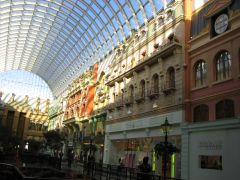
\includegraphics[width=.45\linewidth]{gfx/example_1}} \quad
%\subfloat[Pan ma signo.]
%{\label{fig:example-b}
%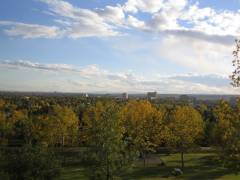
\includegraphics[width=.45\linewidth]{gfx/example_2}} \\
%\subfloat[Methodicamente o uno.]
%{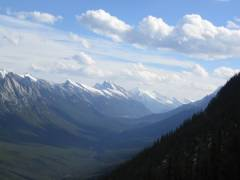
\includegraphics[width=.45\linewidth]{gfx/example_3}} \quad
%\subfloat[Titulo debitas.]
%{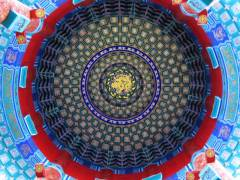
\includegraphics[width=.45\linewidth]{gfx/example_4}}
%\caption[Tu duo titulo debitas latente]{Tu duo titulo debitas latente.}\label{fig:example}
%\end{figure} % Chapter 2
%% Chapter 3

\chapter{Math Test Chapter} % Chapter title

\label{ch:mathtest} % For referencing the chapter elsewhere, use \autoref{ch:mathtest}

%----------------------------------------------------------------------------------------

%\lipsum[13]
%
%%----------------------------------------------------------------------------------------
%
%\section{Some Formulas}
%
%Due to the statistical nature of ionisation energy loss, large fluctuations can occur in the amount of energy deposited by a particle traversing an absorber element\footnote{Examples taken from Walter Schmidt's great gallery: \\ \url{http://home.vrweb.de/~was/mathfonts.html}}.  Continuous processes such as multiple scattering and energy loss play a relevant role in the longitudinal and lateral development of electromagnetic and hadronic showers, and in the case of sampling calorimeters the measured resolution can be significantly affected by such fluctuations in their active layers.  The description of ionisation fluctuations is characterised by the significance parameter $\kappa$, which is proportional to the ratio of mean energy loss to the maximum allowed energy transfer in a single collision with an atomic electron: \graffito{You might get unexpected results using math in chapter or section heads. Consider the \texttt{pdfspacing} option.}
%\begin{equation}
%\kappa =\frac{\xi}{E_{\mathrm{max}}} %\mathbb{ZNR}
%\end{equation}
%$E_{\mathrm{max}}$ is the maximum transferable energy in a single collision with an atomic electron.
%\[E_{\mathrm{max}} =\frac{2 m_{\mathrm{e}} \beta^2\gamma^2 }{1 + 2\gamma m_{\mathrm{e}}/m_{\mathrm{x}} + \left ( m_{\mathrm{e}} /m_{\mathrm{x}}\right)^2}\ ,\]
%where $\gamma = E/m_{\mathrm{x}}$, $E$ is energy and $m_{\mathrm{x}}$ the mass of the incident particle, $\beta^2 = 1 - 1/\gamma^2$ and $m_{\mathrm{e}}$ is the electron mass. $\xi$ comes from the Rutherford scattering cross section and is defined as:
%\begin{eqnarray*} \xi  = \frac{2\pi z^2 e^4 N_{\mathrm{Av}} Z \rho
%\delta x}{m_{\mathrm{e}} \beta^2 c^2 A} =  153.4 \frac{z^2}{\beta^2}
%\frac{Z}{A}
%\rho \delta x \quad\mathrm{keV},
%\end{eqnarray*}
%where
%
%\begin{tabular}{ll}
%$z$ & charge of the incident particle \\
%$N_{\mathrm{Av}}$ & Avogadro's number \\
%$Z$ & atomic number of the material \\
%$A$ & atomic weight of the material \\
%$\rho$ & density \\
%$ \delta x$ & thickness of the material \\
%\end{tabular}
%
%$\kappa$ measures the contribution of the collisions with energy transfer close to $E_{\mathrm{max}}$.  For a given absorber, $\kappa$ tends towards large values if $\delta x$ is large and/or if $\beta$ is small.  Likewise, $\kappa$ tends towards zero if $\delta x $ is small and/or if $\beta$ approaches $1$.
%
%The value of $\kappa$ distinguishes two regimes which occur in the description of ionisation fluctuations:
%
%\begin{enumerate}
%\item A large number of collisions involving the loss of all or most of the incident particle energy during the traversal of an absorber.
%
%As the total energy transfer is composed of a multitude of small energy losses, we can apply the central limit theorem and describe the fluctuations by a Gaussian distribution. This case is applicable to non-relativistic particles and is described by the inequality $\kappa > 10 $ (\ie, when the mean energy loss in the absorber is greater than the maximum energy transfer in a single collision).
%
%\item Particles traversing thin counters and incident electrons under any conditions.
%
%The relevant inequalities and distributions are $ 0.01 < \kappa < 10 $, Vavilov distribution, and $\kappa < 0.01 $, Landau distribution.
%\end{enumerate}
%
%%----------------------------------------------------------------------------------------
%
%\section{Various Mathematical Examples}
%
%If $n > 2$, the identity \[t[u_1,\dots,u_n] = t\bigl[t[u_1,\dots,u_{n_1}], t[u_2,\dots,u_n] \bigr]\] defines $t[u_1,\dots,u_n]$ recursively, and it can be shown that the alternative definition \[t[u_1,\dots,u_n] = t\bigl[t[u_1,u_2],\dots,t[u_{n-1},u_n]\bigr]\] gives the same result. % Chapter 3
%% Chapter 4

\chapter{Analysis} % Chapter title

\label{ch:analysis} % For referencing the chapter elsewhere, use \autoref{ch:mathtest}

In this chapter, we will perform different distributional analyses on the extracted propositions regarding a variety of aspects to gain further insights. We will initially give an overview of the nature and distribution of the extracted propositions as well as evaluate the productivity of the patterns that produced them.
Subsequently, we will compare two association metric frequently employed in sentiment analysis, point-wise mutual information (PMI) and chi-square, for their use in determining ngrams that are most associated with an emotion. We briefly compare the salience of emotion unigrams and bigrams, before we compare the prior probability of association with an emotion for the following configurations of the emotion holder and cause: \begin{inparaenum}[(a)] [\itshape a\upshape)] \item emotion holder; \item NP cause; \item S cause subject + predicate; and \item S cause predicate + object. \end{inparaenum} To this end, we use two evaluation methods: \begin{inparaenum}[(a)] [\itshape a\upshape)] \item We match our bigrams against annotations in the emotion lexicon EmoLex \cite{nrc_emolex} that we presented in chapter \ref{ch:patterns} section \ref{sec:emolex} to obtain an initial guidance. \item Secondly, we let human annotators annotate the most promising configurations of bigrams to obtain a gold standard that we use for evaluation. \end{inparaenum} Finally, an extension of Latent Dirichlet Allocation (LDA) that allows the introduction of supervised category information enables us to generate topics that are associated with our emotions. We investigate different topic configurations and intrinsically evaluate these topics using EmoLex.

\section{Extraction results}

Matching the patterns against the whole annotated Gigaword corpus, we're able to retrieve 2,320,636 extractions. These extractions, however, contain many duplicates, e.g. the sentence "In 1997, with only three years as Texas governor, Bush raised a record-sized warchest that scared away several challengers and found himself at the top of polls of potential 2000 GOP candidates." occurs in the annotated Gigaword file \textsc{apw\_eng\_200011.xml.gz} 25 times in different documents.

After removing all extractions that stem from identical sentences, we arrive at 1,788,022 extractions. After an investigation of the results, we decided to remove extractions with the following patterns from the corpus as they may often refer to unemotive contexts in the news domain that are different from the ones we originally intended:

\begin{itemize}
	\item \textit{grate}: Although occasionally used emotively, \textit{grate} is most often used in an unemotive context related to cooking.
	\item \textit{depress}: As economics are a frequent topic, \textit{depress} often refers to sales or prices rather than the mental state of persons.
	\item \textit{aggravate}: In international politics, \textit{aggravate} often relates to conditions instead of individuals.
	\item \textit{rattle}: In politics, someone may \textit{rattle off} an argument or an earthquake may \textit{rattle} a city.
	\item \textit{afflict}: An ailment often \textit{afflicts} people.
	\item \textit{inflame}: \textit{Inflame} is often used metaphorically, i.e. \textit{inflame} the bonfire of terrorism, the spirit of war, etc.
\end{itemize}

\begin{table}[h]
\centering
\begin{tabular}{l|r|r|r}
{\bf Emotion} & {\bf Frequency} & {\bf\% of total extractions} & {\bf\# of patterns with}\\
              &                 &                              & {\bf 10+ occurrences}\\\hline
anticipation  & 966,571          & 54.47                       & 22 \\
fear          & 249,103          & 14.04                       & 20 \\
joy           & 231,967          & 13.07                       & 30 \\
trust         & 89,217           & 5.03                        &  6 \\
anger         & 64,586           & 3.64                        & 28 \\
surprise      & 60,221           & 3.39                        & 20 \\
disgust       & 59,486           & 3.35                        & 15 \\
sadness       & 53,269           & 3.00                        & 13\\\hline
Total         & 1,774,420         & 100.00                     & 154                
\end{tabular}
\caption{Frequencies of emotions in extractions}
\label{tab:extraction-emotion-freq}
\end{table}

Excluding these patterns in their active and passive forms leaves us with 1,774,420 distinct extractions. Their emotion distribution is depicted in table \ref{tab:extraction-emotion-freq}, while the distribution of nominal phrases and clauses as causes can be viewed in table \ref{tab:patterns-np-vs-s}. As can be seen, anticipation makes up slightly more than half of all extractions, which is mainly due to \textit{expect} being a very productive pattern, as depicted in table \ref{tab:anticipation-patterns}.

\begin{table}[h]
\centering
\begin{tabular}{l|r|r}
{\bf Emotion} & {\bf \# extractions} & {\bf \# extractions} \\
{\bf }        & {\bf with NP cause}         & {\bf with S cause}          \\\hline
anticipation  & 407,738 & 558,833                \\
joy           & 190,484 & 41,483                 \\
fear          & 82,116 & 166,987                \\
trust         & 72,483 & 16,734                 \\
surprise      & 59,657 & 564                    \\
disgust       & 58,942 & 544                    \\
anger         & 57,379 & 7,207                  \\
sadness       & 26,064 & 27,205                 \\\hline
Total         & 956,392 &	819,557
\end{tabular}
\caption{Patterns with NP vs. S cause}
\label{tab:patterns-np-vs-s}
\end{table}

Due to space requirements, we display the top 10 patterns for each of Plutchik's eight emotions and discuss them briefly.

\begin{table}[!htb]
    \begin{minipage}{.45\linewidth}
		\centering
		\begin{tabular}{l|r}
			{\bf Pattern} & {\bf Frequency} \\\hline
			surprise      & 18,358          \\
			stun          & 16,211          \\
			shock         & 13,269          \\
			confuse       & 2,899           \\
			wow           & 2,003           \\
			confound      & 1,771           \\
			startle       & 1,680           \\
			baffle        & 1,169           \\
			puzzle        & 802             \\
			stagger       & 689             \\\hline
			Total top 10  & 58,851          \\
			Total         & 60,221         
		\end{tabular}
		\caption{Top 10 surprise patterns}
		\label{tab:surprise-patterns}
	\end{minipage}
	\begin{minipage}{.45\linewidth}
		\centering
		\begin{tabular}{l|r}
			{\bf Pattern}   & {\bf Frequency} \\\hline
			expect          & 490,640         \\
			predict         & 156,681         \\
			await           & 71,910          \\
			look forward to & 59,884          \\
			prepare for     & 45,687          \\
			forecast        & 45,365          \\
			hope            & 28,277          \\
			anticipate      & 19,112          \\
			be hopeful      & 17,732          \\
			foresee         & 9,248           \\\hline
			Total top 10    & 944,536         \\
			Total           & 966,571        
		\end{tabular}
		\caption{Top 10 anticipation patterns}
		\label{tab:anticipation-patterns}
	\end{minipage}
\end{table}

\begin{table}[!htb]
    \begin{minipage}{.45\linewidth}
    		\centering
		\begin{tabular}{l|r}
			{\bf Pattern} & {\bf Freq} \\\hline
			enjoy         & 131,102         \\
			be proud      & 21,842          \\
			be lucky      & 13,857          \\
			cheer         & 10,658          \\
			relish        & 5,590           \\
			impress       & 5,431           \\
			entertain     & 4,318           \\
			arouse        & 4,247           \\
			be satisfied  & 4,016           \\
			please        & 3,394           \\\hline
			Total top 10  & 204,455         \\
			Total         & 231,967        
		\end{tabular}
		\caption{Top 10 joy patterns}
		\label{tab:joy-patterns}
	\end{minipage}
    	\begin{minipage}{.45\linewidth}
      	\centering
		\begin{tabular}{l|r}
			{\bf Pattern} & {\bf Freq} \\\hline
			regret        & 24,395          \\
			mourn         & 7,948           \\
			be unhappy    & 6,120           \\
			be sad        & 5,071           \\
			disappoint    & 3,320           \\
			upset         & 2,439           \\
			grieve        & 1,317           \\
			pine for      & 1,064           \\
			agonize over  & 489             \\
			displease     & 423             \\\hline
			Total top 10  & 52,586          \\
			Total         & 53,269          
		\end{tabular}
	\caption{Top 10 sadness patterns}
	\label{tab:sadness-patterns}
    \end{minipage}
\end{table}

\begin{table}[!htb]
    \begin{minipage}{.45\linewidth}
		\centering
		\begin{tabular}{l|r}
			{\bf Pattern}   & {\bf Freq} \\\hline
			rely on         & 50,480          \\
			count on        & 17,562          \\
			trust           & 14,749          \\
			reassure        & 5,384           \\
			take comfort in & 620             \\
			charm           & 412             \\
			be charmed      & 7               \\
			be reassured    & 3               \\
			                &                 \\
			                &                 \\\hline
			Total top 10    & 89,217          \\
			Total           & 89,217         
		\end{tabular}
		\caption{Top 10 trust patterns}
		\label{tab:trust-patterns}
    \end{minipage}
    \begin{minipage}{.45\linewidth}
		\centering
		\begin{tabular}{l|r}
			{\bf Pattern} & {\bf Freq} \\\hline
			hate          & 22,804          \\
			shun          & 9,268           \\
			deplore       & 8,751           \\
			dislike       & 6,069           \\
			alienate      & 2,675           \\
			repel         & 2,054           \\
			despise       & 1,828           \\
			loathe        & 1,328           \\
			disdain       & 1,208           \\
			abhor         & 1,149           \\\hline
			Total top 10  & 57,134           \\
			Total         & 59,486          
		\end{tabular}
		\caption{Top 10 disgust patterns}
		\label{tab:disgust-patterns}
    \end{minipage}
\end{table}

\begin{table}[!htb]
    \begin{minipage}{.45\linewidth}
		\centering
		\begin{tabular}{l|r}
			{\bf Pattern} & {\bf Frequency} \\\hline
			fear          & 155,968         \\
			be afraid     & 35,314          \\
			worry         & 25,361          \\
			be anxious    & 10,427          \\
			scare         & 6,704           \\
			be scared     & 3,340           \\
			be nervous    & 2,195           \\
			frighten      & 1,992           \\
			unnerve       & 1,573           \\
			dread         & 1,534           \\\hline
			Total top 10  & 244,408         \\
			Total         & 249,103        
		\end{tabular}
		\caption{Top 10 fear patterns}
		\label{tab:fear-patterns}
	\end{minipage}
    \begin{minipage}{.45\linewidth}
		\centering
		\begin{tabular}{l|r}
			{\bf Pattern} & {\bf Frequency} \\\hline
			provoke       & 16,528          \\
			be angry      & 6,808           \\
			bother        & 6,612           \\
			infuriate     & 5,316           \\
			harass        & 4,791           \\
			insult        & 3,534           \\
			frustrate     & 2,912           \\
			irritate      & 2,805           \\
			offend        & 2,482           \\
			fret          & 2,356           \\\hline
			Total top 10  & 54,144          \\
			Total         & 64,586         
		\end{tabular}
		\caption{Top 10 anger patterns}
		\label{tab:anger-patterns}
	\end{minipage}
\end{table}

Analogous to social media data, which has been found to be predominantly happy \cite{depechemood} due to its subjectivity, neutral predicates are prevalent given the idiosyncracies of the objective news domain. Consequently, anticipation as well as neutral predicates such as \textit{expect}, \textit{predict}, and \textit{rely on} rank highly. Additionally, \textit{enjoy} and \textit{fear} are very productive, which seem to be the preferred ways to indicate the polar opposites of joy and fear. As is according to style conventions of news texts and creative writing, passive forms play a subordinate role and are (except for trust, which had less than ten patterns) not found in the top ten patterns of any emotion. When we look at the distribution between NP causes and S causes between emotions in table \ref{tab:patterns-np-vs-s}, we see that -- except for anticipation and fear -- NP causes dominate -- and quite clearly in the cases of surprise, disgust, and anger. This is due to the prevalent use of the active form of Experiencer psych verbs such as \textit{surprise}, \textit{hate}, \textit{provoke}, etc. which predominantly take a nominal phrase as their argument.
	
\section{Distributional analysis of emotion holder and cause}

For the distributional analysis of the results, we first count the occurrences of all unigrams and bigrams respectively for the emotion holder, the NP cause, the S cause as well as the predicate of the S cause together with the subject and together with the object respectively. To guarantee maximum meaningfulness of the results, we treat prepositional objects as one unigram. We convert all ngrams to lowercase if they are not named entities; for named entities, we keep the NE tags in a shortened form for better readability; finally, we remove all stopwords.

We generate unigrams for the following strings:
\begin{aenumerate}
	\item The emotion holder
	\item The NP cause
	\item The whole S cause
\end{aenumerate}

We generate bigrams for the above as well as the following strings:
\begin{aenumerate}
	\item The subject of the S cause concatenated with its predicate
	\item The predicate of the S cause concatenated with its object
\end{aenumerate}

In both of the latter, the predicate is always part of the bigram. The counts of number of unigrams and bigrams for the different configurations can be found in \ref{tab:unigram_bigram_count_ngram_type}. We observe unigram counts around 2m, while bigram counts range around 1m, except for the predicate + direct object configuration.

\begin{table}[h]
\centering
\begin{tabular}{l|r|r}
{\bf Ngram type}      & {\bf \# unigrams} & {\bf \# bigrams} \\\hline
Subj + Pred (S cause) & 0                 & 921,337          \\
NP cause              & 1,856,712         & 915,122          \\
Pred + Dobj (S cause) & 0                 & 168,013          \\
S cause               & 2,307,214         & 1,490,232        \\
Emotion holder        & 2,809,796         & 1,279,699       
\end{tabular}
\caption{Number of unigrams and bigrams for different emotion holder / cause configurations}
\label{tab:unigram_bigram_count_ngram_type}
\end{table}

We use two association metrics that have been used frequently in sentiment analysis: pointwise mutual information (PMI) and chi-square.

\subsection{PMI}

PMI, which is derived from information theory, models the mutual information between two expressions. The PMI for two expressions $x$ and $y$ is defined as the ratio of their joint probability and the product of their individiual probabilities:

$$pmi(x;y) = log \dfrac{p(x,y)}{p(x)p(y)}$$

with $p(x,y) = \frac{f(x;y)}{N}$ and $p(x)p(y) = \frac{f(x)f(y)}{N^{2}}$, where $f(x)$ is the frequency of $x$ in the corpus and $N$ is the number of extractions.

$x$ and $y$ are associated with each other, if their PMI is greater than 0 -- with their association strength increasing with the PMI score; they are negatively associated if their PMI is less than 0.
In our case, $x$ is the emotion and $y$ is a unigram or bigram that occurs with the emotion.

The regular PMI measure has one issue in that if $y$ occurs just once with emotion $x$ and with no other emotion, $p(x,y) = p(y)$, which reduces the above equation to $pmi(x;y) = log \frac{1}{p(x)}$, which is independent of the ngram $y$ as it is just the probability of emotion $x$.

\citeauthor{twitter_hashtags_nrc} simply ignore ngrams that occur less than five times, which, however, only unsatisfactorily mitigates the issue. Instead, in order to penalize such low-frequency observations, we use a simple discounting method that has been described by \citeauthor{pmi_discount} and already put to you use by \citeauthor{matt_dissertation_pmi}. Multiplying the numinator with the discount factor produces the following term:

$$\frac{f(x;y)}{N} \cdot \frac{f(x;y)}{f(x;y) + 1}$$

If the ngram occurs very rarely, the discount factor will be small, reducing the PMI score. We apply a similar discount to the denominator, which reduces to the n-gram frequency divided by the n-gram frequency + 1, as the ngram would always occur less often than the associated emotion category:

$$\frac{f(x)f(y)}{N^{2}\frac{min(f(x),f(y)}{min(f(x),f(y) + 1})} = \frac{f(x)f(y)}{N^{2}\frac{f(y)}{f(y) + 1}}$$

If the ngram is rarely observed, $ \frac{f(y)}{f(y) + 1} $ is small, making the denominator large, which reduces the PMI score. In general, the discount factor reduces the PMI score for ngrams that are very infrequent ($f(y)$ close to 1) and minimally impacts all other PMI scores -- which is exactly the behaviour that we want.

Another common variant of the PMI measure is the normalized PMI score, which restricts the PMI value to the interval $[-1,+1]$, where -1 signifies no joint occurrence, 0 is independence, and +1 represents complete co-occurrence. We have experimentally applied this, but found that it negates the effect of the introduced discount, which led us to decide against its use.

\subsection{Chi-square}

Chi-square ($\chi^{2}$) is another common measure. Let $n$ be the number of all documents, i.e. extractions, $p(x|y)$ be the conditional probability of emotion $x$ occurring with ngram $y$, $P(x)$ be the fraction of extractions containing emotion $x$, and $F(y)$ be the fraction of extractions containing ngram $y$, which we define as follows:

$$p(x|y) = \frac{p(x;y)}{p(y)}$$

$$P(x) = \frac{f(x)}{n}$$

$$F(y) = \frac{f(y)}{n}$$

With these, the $\chi^{2}$ metric between emotion $x$ and ngram $y$ is defined as \cite{chi-square}: 

$$\chi^{2} = \frac{n \cdot F(y)^{2} \cdot (p(x|y) - P(x))^{2}}{F(y) \cdot (1 - F(y)) \cdot P(x) \cdot (1 - P(x))}$$

$\chi^{2}$ and PMI are two different ways of measuring how well a term and a category correlate. $\chi^{2}$ in contrast to PMI is a normalized value, making it more comparable across the same category. $\chi^{2}$, however, doesn't penalize infrequent terms, which the discounted PMI score does. We compare the results of the PMI and $\chi^{2}$ metrics for an initial set of results and then proceed with the metric that yields the better performance.

\subsection{PMI vs. chi-square}

We clearly want to be able to compare values not only among the different types of unigrams and bigrams that we extract but also across different emotions. If we compare the PMI values of top bigrams in the NP cause of different emotions, we find that their range lends itself to easy comparison, with the top 10,000 bigrams of each emotion falling in an interval between 3.40 (sadness) and 0.16 (surprise) as depicted in figure \ref{fig:pmi distribution}.

\begin{figure}[bth]
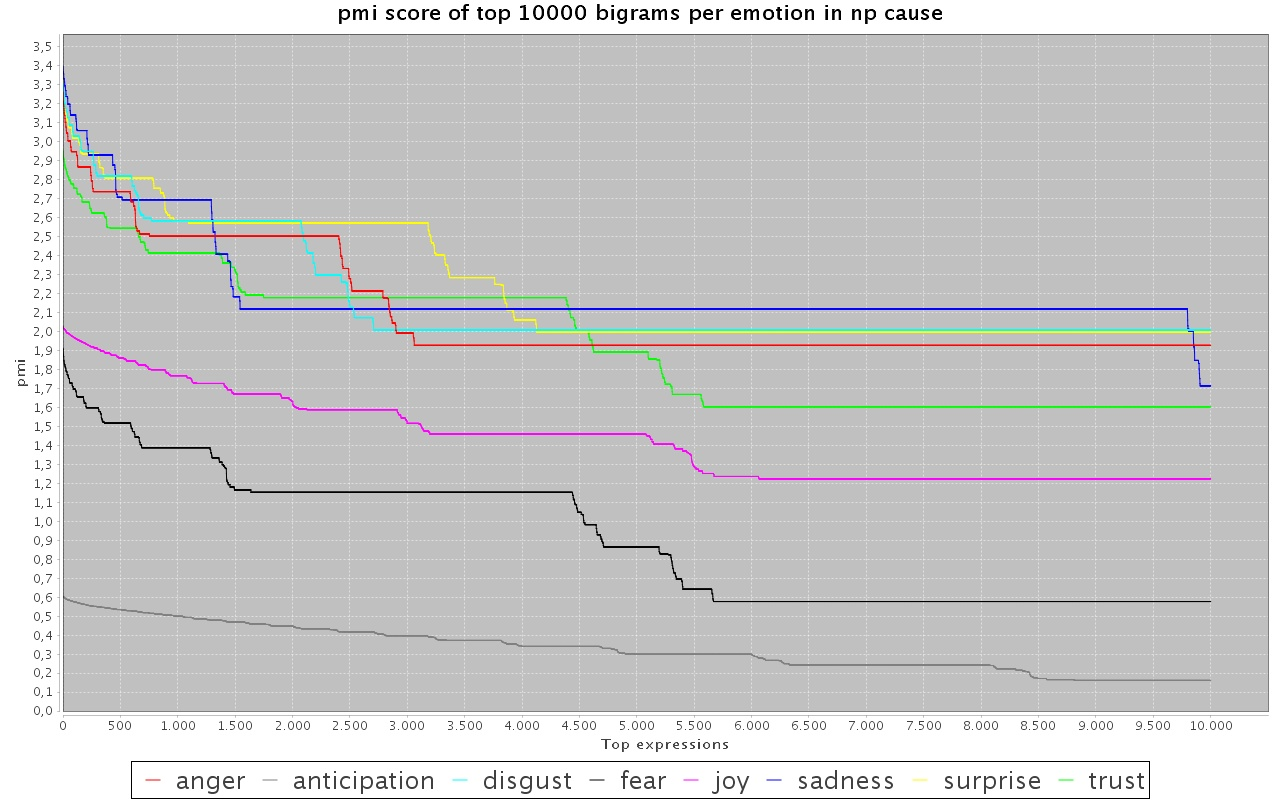
\includegraphics[width=\linewidth]{gfx/pmi_bigram_np_cause_comparison_10000.jpg}
\caption{PMI values for the top 10,000 bigrams for each emotion}\label{fig:pmi distribution}
\end{figure}

Conversely, $\chi^{2}$ values, whose distribution ranges from 9,426 (sadness) to 73.68 (fear) for the top 100 bigrams of each emotion -- as can be seen in figure \ref{fig:chi-square distribution} -- renders comparison of $\chi^{2}$ values across emotions moot.

\begin{figure}[bth]
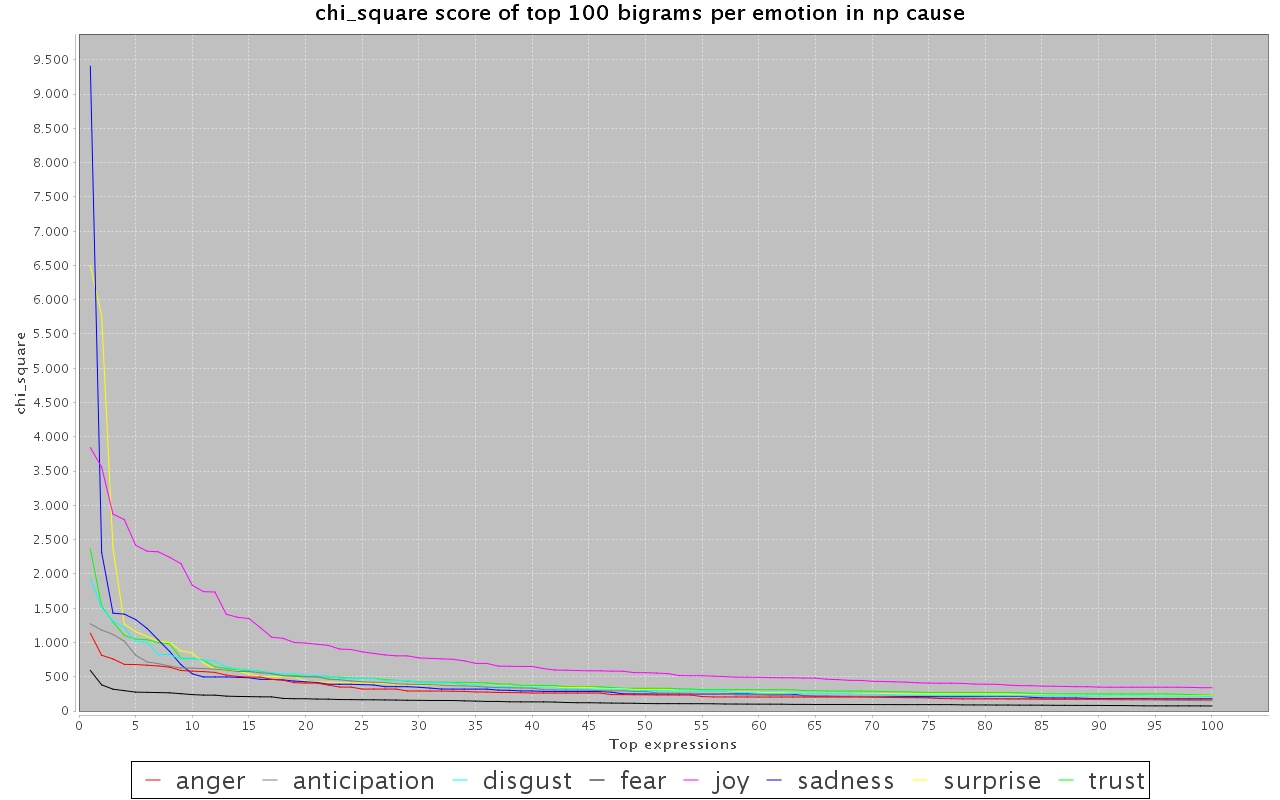
\includegraphics[width=\linewidth]{gfx/chi_square_bigram_np_cause_comparison_100.jpg}
\caption{$\chi^{2}$ values for the top 100 bigrams}\label{fig:chi-square distribution}
\end{figure}

Comparing the top 10 NP cause bigrams of sadness, the emotion with the top-ranked bigram for each measure, in table \ref{tab:chi-pmi sadness} shows that both measures produce sensible candidates. Among $\chi^{2}$ sadness bigrams, the theme of \textit{loss} is prevalent, while among PMI bigrams \textit{death} dominates. PMI bigrams are also grouped much more closely, while the huge gap between the first and second $\chi^{2}$ candidate isn't plausibly justifiable.

\begin{table}[h]
\centering
\begin{tabular}{l|r|l|r}
{\bf $\chi^{2}$ bigram} & {\bf $\chi^{2}$ value} & {\bf PMI bigram}        & {\bf PMI value} \\\hline
loss of:life            & 9426.09                & death of:NUM         & 3.40            \\
loss of:innocent\_life  & 2317.45                & quake victim            & 3.37            \\
tragic loss             & 1430.38                & death of:wife           & 3.37            \\
loss of:civilian\_life  & 1416.05                & loss of:man             & 3.37            \\
civilian casualty       & 1303.09                & tragic loss             & 3.36            \\
death of:NUM            & 1208.49                & death of:father         & 3.36            \\
death of:NUM\_people & 1038.87                & death of:NUM\_people & 3.34            \\
NUM victim           & 870.43                 & death of:relative       & 3.33            \\
unfortunate incident    & 677.81                 & loss of:friend          & 3.33            \\
choice of:word          & 516.71                 & innocent victim         & 3.33           
\end{tabular}
\caption{Comparison of $\chi^{2}$ and PMI values for the top 10 sadness NP cause bigrams}
\label{tab:chi-pmi sadness}
\end{table}

In light of the lack of comparability across emotions and the semantically injustifiable huge differences for the same emotion with the $\chi^{2}$ measure and given length constraints, we choose to proceed with further analyses using the PMI metric.

\subsection{Bigrams vs. unigrams}

Having seen the top 10 NP cause sadness bigrams, when we take a look at the corresponding unigrams in table \ref{tab:sadness-unigrams}, we find that, while a lot of them are plausible, units like \textit{to:embassy}, \textit{of:grandson}, or \textit{of:Princess\_Diana/PERS} are totally inconsequential without the relevant context. Note that \textit{uday} -- actually Uday Hussein -- was erroneously tagged as \textsc{VBP}.

\begin{table}[h]
\centering
\begin{tabular}{l|r}
{\bf Unigram}                                    & {\bf PMI score} \\\hline
inconvenience                                    & 3.43            \\
misunderstanding                                 & 3.42            \\
passing                                          & 3.32            \\
to:embassy                                       & 3.32            \\
slay                                             & 3.28            \\
of:grandson                                      & 3.27            \\
assassinate                                      & 3.27            \\
of:Princess\_Diana/PERS                          & 3.25            \\
error                                            & 3.25            \\
uday                                             & 3.24              
\end{tabular}
\caption{Top 10 NP cause sadness unigrams}
\label{tab:sadness-unigrams}
\end{table}

In order to avoid errors in further analyses, we focus on bigrams instead of unigrams, as they are more meaningful without context.

\subsection{Ambiguous concepts}

Before investigating individual emotions, we take a look at the most ambiguous bigrams, those who have the highest PMI score summed across all emotions. The top 20 NP cause bigrams are displayed in table \ref{tab:percent-bigrams-overlap-pmi}, with each emotion's portion of the overall PMI score depicted in percent. The same information is displayed in absolute PMI scores for the top 50 bigrams in figures \ref{fig:pmi-bigram-np-cause-emotion-overlap-50} and \ref{fig:pmi-bigram-np-cause-sentiment-overlap-50} across emotions and sentiment respectively. 
Interestingly, anticipation and fear don't appear among the most ambiguous bigrams.

\begin{table}[h]
\centering
\begin{tabular}{l|r|r|r|r|r|r}
{\bf Bigram} & {\bf anger} & {\bf disgust} & {\bf joy} & {\bf sadness} & {\bf surprise} & {\bf trust} \\\hline
former president & 21.09 & 28.12 & 0.79 & 20.74 & 25.46 & 3.81 \\
prime minister & 28.50 & 11.05 & 0.00 & 2.71 & 31.20 & 26.53 \\
shoot death & 27.55 & 20.80 & 0.00 & 31.05 & 20.60 & 0.00 \\
United/LOC States/LOC & 19.35 & 34.57 & 0.00 & 0.00 & 25.77 & 20.31 \\
hostage crisis & 29.78 & 22.87 & 0.00 & 24.69 & 22.66 & 0.00 \\
president Chen/PERS & 41.25 & 32.82 & 0.00 & 0.00 & 19.22 & 6.72 \\
president Clinton/PERS & 27.69 & 32.52 & 1.43 & 11.26 & 13.96 & 13.16 \\
Tony/PERS Blair/PERS & 21.51 & 28.01 & 0.00 & 0.00 & 25.61 & 24.87 \\
police officer & 34.97 & 18.29 & 0.00 & 2.19 & 34.56 & 9.99 \\
president George/PERS & 21.21 & 25.61 & 1.68 & 0.00 & 26.18 & 25.32 \\
Israeli/LOC prime & 30.29 & 0.00 & 0.00 & 12.08 & 37.24 & 20.39 \\
Boris/PERS Yeltsin/PERS & 0.00 & 19.69 & 0.00 & 13.78 & 43.14 & 23.39 \\
security guard & 16.49 & 42.61 & 0.00 & 0.00 & 18.10 & 22.79 \\
russian troops & 14.11 & 33.98 & 0.00 & 0.00 & 26.94 & 24.98 \\
minister Tony/PERS & 25.29 & 23.48 & 0.00 & 0.00 & 23.27 & 27.96 \\
president Jacques/PERS & 36.64 & 15.50 & 0.00 & 21.97 & 9.19 & 16.69 \\
Rudolph/PERS Giuliani/PERS & 30.31 & 32.14 & 0.00 & 0.00 & 37.54 & 0.00 \\
W./PERS Bush/PERS & 14.72 & 30.69 & 4.48 & 1.38 & 25.89 & 22.84 \\
Saudi/LOC Arabia/LOC & 25.35 & 0.00 & 0.00 & 9.31 & 38.51 & 26.83
\end{tabular}
\caption{Emotion distribution in \% of top 20 NP cause bigrams with highest aggregated PMI score; \textit{fear} and \textit{anticipation} have 0 PMI for all instances}
\label{tab:percent-bigrams-overlap-pmi}
\end{table}

Named entities like state leaders and states are among the most polarizing concepts. Even regarding these political powers, PMI scores of the neutral anticipation -- essentially the most common emotion in politics -- are negative, emphasizing the genericity and vagueness of Plutchik's anticipation and underlining why it isn't used in other classifications
\cite{ekman_basic_emotions}.

If we ignore named entities, expressions that are associated with violence such as \textit{shooting death} and \textit{hostage crisis} or that may potentially be deployed controversially such as \textit{police officer}, \textit{security guard}, and \textit{Russian troops} possess the highest aggregated scores. Trust is placed in the \textit{Russian troops} e.g. by "Tajikistan 's hard-line government", which relied on them in 1998 "to guard the Afghan border against incursions by guerillas and smugglers" (\texttt{APW\_ENG\_19980116.0782/13}). The capability to showcase the development of such emotive trends over time thus presents an interesting research opportunity and will produce further insights on how public opinion on certain concepts fares. Date information can be easily extracted from the extraction ID; as an investigation of the temporal aspect would significantly inflate the scope of this project, we will leave it for future work.

Interestingly, even among such potentially violent concepts as the ones mentioned above, PMI scores for fear are still negative. Conversely, the top 10 NP cause bigrams that have the highest fear PMI scores (cf. \ref{ch:appendix}, table \ref{tab:pmi-fear-np-cause-10}) all spread fear on a national level, while the above mentioned concepts would be condemned by the general public rather than scare it.

Finally, considering the two expressions ranked as the most ambiguous, \textit{former president} and \textit{prime minister}, both of them can refer to leader of states that are objects of a diversity of emotions, e.g. "South Korea's former president Roh" (\texttt{AFP\_ENG\_20090528.0118/7}) is mourned by thousands, while Washington loathes "two (corrupt) former presidents (of Nicaragua)" (\texttt{APW\_ENG\_20051205.0005/5}). Even former leader's decisions may still evoke expressions of anger or surprise, but the media will be more cautious with signs of the stronger disgust for current than for former leaders. Furthermore, the degree of anteriority implied by \textit{former president} is linked to sadness, whereas support will rather be given to a current leader.

\begin{figure}[bth]
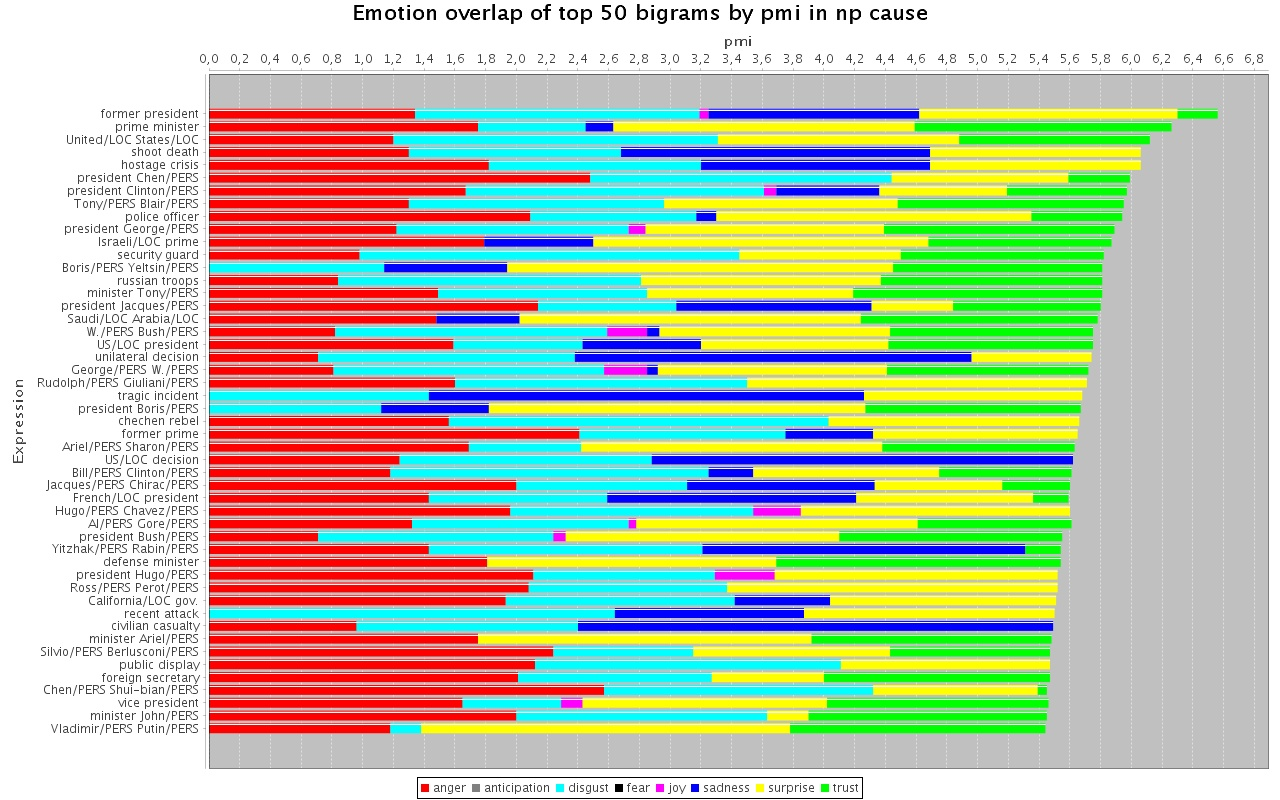
\includegraphics[width=\linewidth]{gfx/pmi_bigram_np_cause_emotion_overlap_50.jpg}
\caption{Overlap across emotions for the top 50 PMI NP cause bigrams}\label{fig:pmi-bigram-np-cause-emotion-overlap-50}
\end{figure}

\begin{figure}[bth]
\includegraphics[width=\linewidth]{gfx/pmi_bigram_np_cause_sentiment_overlap_50.jpg}
\caption{Overlap across sentiment for the top 50 PMI NP cause bigrams}\label{fig:pmi-bigram-np-cause-sentiment-overlap-50}
\end{figure}

Considering the entirety of ambiguous expressions displayed in figure \ref{fig:pmi-bigram-np-cause-emotion-overlap-50}, we observe that degrees of anger (\textit{red}), disgust (\textit{cyan}), and surprise (\textit{yellow}) are present in almost all concepts. Trust (\textit{green}) frequently appears as well, sadness (\textit{blue}) less often, although more dominantly if it does, while joy (\textit{magenta}) is hardly visible. All in all, negative sentiment (\textit{red}) prevails as seen in figure \ref{fig:pmi-bigram-np-cause-sentiment-overlap-50}.

\subsection{Emotion holder vs. cause configurations} \label{sec:emolex-evaluation}

We have previously mentioned the NRC Word-Emotion Association Lexicon (EmoLex) \cite{nrc_emolex}. We weren't able to use it for our collection of patterns; we will, though, utilize it in order to partially validate association with an emotion for our concepts. We will initially compare the overlap of the different configurations of bigrams at hand with EmoLex to evaluate which bigrams we will examine more closely in our subsequent human-annotated evaluation.

\begin{inparaenum}[(a)] [\itshape a\upshape)] We will compare at this point bigrams from \item the emotion holder, \item the NP cause, \item the S cause subject and predicate, and \item the S cause predicate and object \end{inparaenum}. As the predicate of the complement is the most meaningful part in a clausal cause, it is always present in the two latter bigrams. We initially calculate the PMI scores for all emotions for all bigram configurations, excluding all bigrams that contain a named entity as these are not present in EmoLex. In order to allow a We select the top 30 bigrams per emotion per configuration and calculate a ternary overlap with EmoLex: As EmoLex only contains unigrams, we assign \texttt{NA} (\textit{grey}) if none of the unigrams of the bigram appears in EmoLex; if one of them appears in EmoLex with the respective emotion, we assign \texttt{TRUE} (\textit{green}); otherwise we assign \texttt{FALSE}. As EmoLex also contains a label for \textit{positive} and \textit{negative}, we also calculate the sentiment overlap by mapping our emotions to its sentiment (see table \ref{tab:emotion2sentiment}) and checking if it appears with the respective sentiment in EmoLex as above. 

\begin{table}[]
\centering
\begin{tabular}{l|l||l|l}
{\bf Emotion} & {\bf Sentiment} & {\bf Emotion} & {\bf Sentiment} \\\hline
anticipation  & neutral         & anger         & negative        \\
surprise      & neutral         & fear          & negative        \\
joy           & positive        & disgust       & negative        \\
trust         & positive        & sadness       & negative       
\end{tabular}
\caption{Mapping of emotions to sentiment}
\label{tab:emotion2sentiment}
\end{table}

We show the results in tables \ref{tab:emotion-holder-nrc-overlap}, \ref{tab:s-cause-subj-pred-nrc-overlap}, \ref{tab:s-cause-pred-dobj-nrc-overlap}, and \ref{tab:np-cause-nrc-overlap}. We include figure \ref{fig:pmi-np-cause-nrc-overlap} exemplarily to visualize the values in table \ref{tab:np-cause-nrc-overlap}. Sentiment columns for anticipation and surprise only contain \texttt{NA} as EmoLex doesn't contain a \textit{negative} label. All numbers are given as percentage of the top 30 bigrams that were chosen for each emotion respectively. Note that percentages for \texttt{TRUE} equal precision. As our \textit{gold standard} for this evaluation, EmoLex, contains 14,000 terms and we only select the 30 bigrams for this evaluation, we don't provide recall nor F-score as they wouldn't add additional insights.

As we've outlined before, emotion is a compositional phenomenon. Thus, this evaluation employing comparison on an unigram-level may only serve as a guideline that will inform further investigation.

Another thing worth remarking is that due to data sparseness for S causes of surprise, disgust, and anger (see table \ref{tab:patterns-np-vs-s}), PMI will frequently not be able to determine reliable candidates, particularly regarding direct objects, which are only present in a subset of the instances.

\begin{table}[]
\centering
\begin{tabular}{l|rr|rr|rr|rr}
{\bf Overlap} & \multicolumn{2}{c}{{\bf anger}} & \multicolumn{2}{c}{{\bf anticipation}} & \multicolumn{2}{c}{{\bf disgust}} & \multicolumn{2}{c}{{\bf fear}} \\
 & {\it Emo} & {\it Sen} & {\it Emo} & {\it Sen} & {\it Emo} & {\it Sen} & {\it Emo} & {\it Sen} \\\hline
\texttt{TRUE} & 46.67 & 50.00 & 10.00 & 0.00 & 6.67 & 53.33 & 10.00 & 20.00 \\
\texttt{NA} & 6.67 & 6.67 & 50.00 & 100.00 & 20.00 & 20.00 & 20.00 & 20.00 \\
\texttt{FALSE} & 46.67 & 43.33 & 40.00 & 0.00 & 73.33 & 26.67 & 70.00 & 60.00 \\
{\bf Overlap} & \multicolumn{2}{c}{{\bf joy}} & \multicolumn{2}{c}{{\bf sadness}} & \multicolumn{2}{c}{{\bf surprise}} & \multicolumn{2}{c}{{\bf trust}} \\
 & {\it Emo} & {\it Sen} & {\it Emo} & {\it Sen} & {\it Emo} & {\it Sen} & {\it Emo} & {\it Sen} \\\hline
\texttt{TRUE} & 3.33 & 30.00 & 3.33 & 6.67 & 0.00 & 0.00 & 13.33 & 10.00 \\
\texttt{NA} & 20.00 & 20.00 & 46.67 & 46.67 & 16.67 & 100.00 & 30.00 & 30.00 \\
\texttt{FALSE} & 76.67 & 50.00 & 50.00 & 46.67 & 83.33 & 0.00 & 56.67 & 60.00
\end{tabular}
\caption{Overlap of the top 30 PMI emotion holder bigrams with EmoLex in \%}
\label{tab:emotion-holder-nrc-overlap}
\end{table}

As can be seen in table \ref{tab:emotion-holder-nrc-overlap}, emotion holder bigrams frequently are not associated with the emotion in EmoLex. This does not surprise, as the experiencer doesn't generally presuppose an emotion, in contrast to the cause of the emotion. The superior precision for anger is due to the fact that \textit{provoke}, the most productive anger pattern, in news frequently refers to inanimate concepts that are -- in fact -- associated with anger, such as \textit{international outcry}, \textit{angry response}, or \textit{international outrage}. 

\begin{table}[]
\centering
\begin{tabular}{l|rr|rr|rr|rr}
{\bf Overlap} & \multicolumn{2}{c}{{\bf anger}} & \multicolumn{2}{c}{{\bf anticipation}} & \multicolumn{2}{c}{{\bf disgust}} & \multicolumn{2}{c}{{\bf fear}} \\\
 & {\it Emo} & {\it Sen} & {\it Emo} & {\it Sen} & {\it Emo} & {\it Sen} & {\it Emo} & {\it Sen} \\\hline
\texttt{TRUE} & 3.33 & 23.33 & 33.33 & 0.00 & 6.67 & 13.33 & 23.33 & 23.33 \\
\texttt{NA} & 16.67 & 16.67 & 3.33 & 100.00 & 50.00 & 50.00 & 36.67 & 36.67 \\
\texttt{FALSE} & 80.00 & 60.00 & 63.33 & 0.00 & 43.33 & 36.67 & 40.00 & 40.00 \\\hline
{\bf Overlap} & \multicolumn{2}{c}{{\bf joy}} & \multicolumn{2}{c}{{\bf sadness}} & \multicolumn{2}{c}{{\bf surprise}} & \multicolumn{2}{c}{{\bf trust}} \\
 & {\it Emo} & {\it Sen} & {\it Emo} & {\it Sen} & {\it Emo} & {\it Sen} & {\it Emo} & {\it Sen} \\\hline
\texttt{TRUE} & 20.00 & 36.67 & 23.33 & 33.33 & 3.33 & 0.00 & 23.33 & 36.67 \\
\texttt{NA} & 30.00 & 30.00 & 6.67 & 6.67 & 30.00 & 100.00 & 23.33 & 23.33 \\
\texttt{FALSE} & 50.00 & 33.33 & 70.00 & 60.00 & 66.67 & 0.00 & 53.33 & 40.00
\end{tabular}
\caption{Overlap of the top 30 PMI S cause subject + predicate bigrams with EmoLex in \%}
\label{tab:s-cause-subj-pred-nrc-overlap}
\end{table}

The low values for anger and disgust in table \ref{tab:s-cause-subj-pred-nrc-overlap} are generally due to data sparseness. EmoLex only inadequately captures the objects of anticipation that are most prominent in news stories: While \textit{grow} as in \textit{gross grow} appears in EmoLex, synonyms like \textit{rise} or \textit{expand} do not. Many fear bigrams can be attributed to viruses and war. While \textit{flu} and \textit{disease} are associated with fear in EmoLex, \textit{virus} is just associated with negative. EmoLex captures bigrams such as \textit{flu mutate} or \textit{war destabilize}, but does not account for equally fearful ones such as \textit{h5n1 mutate}, \textit{virus mutate}, \textit{strain mutate}, or \textit{bird mutate}.
Sports-based joy bigrams such as \textit{team achieve} or \textit{player accomplish} are captured by EmoLex, while others that are only joyful because of their compositionality, e.g. \textit{nobody hurt}, \textit{nobody kill(ed)} are not expressed. Furthermore, our approach captures a lot of terms that are very relevant in politics, such as \textit{condition stabilise}.
A lot of combinations of subjects and predicates are context-dependent. \textit{Situation occur} or \textit{position arise} might be neutral, positive, or negative, but are associated with sadness in the news domain.
Suprise bigrams derived from the S cause and predicate are very ambiguous, due to the neutrality of surprise. Bigrams like \textit{settlement allow} or \textit{anyone object} depend on the context more than anything else to elicit surprise.
Trust bigrams usually refer to the actions of political leaders or powers such as \textit{democrats handle}, \textit{democrats deal}, or \textit{political contribute}. While a few of these are contained in EmoLex, most of them express a partisan trust.

\begin{table}[]
\centering
\begin{tabular}{l|rr|rr|rr|rr}
{\bf Overlap} & \multicolumn{2}{c}{{\bf anger}} & \multicolumn{2}{c}{{\bf anticipation}} & \multicolumn{2}{c}{{\bf disgust}} & \multicolumn{2}{c}{{\bf fear}} \\
 & {\it Emo} & {\it Sen} & {\it Emo} & {\it Sen} & {\it Emo} & {\it Sen} & {\it Emo} & {\it Sen} \\\hline
\texttt{TRUE} & 16.67 & 40.00 & 3.33 & 0.00 & 10.00 & 33.33 & 33.33 & 33.33 \\
\texttt{NA} & 6.67 & 6.67 & 0.00 & 100.00 & 10.00 & 10.00 & 13.33 & 13.33 \\
\texttt{FALSE} & 76.67 & 53.33 & 96.67 & 0.00 & 80.00 & 56.67 & 53.33 & 53.33 \\\hline
{\bf Overlap} & \multicolumn{2}{c}{{\bf joy}} & \multicolumn{2}{c}{{\bf sadness}} & \multicolumn{2}{c}{{\bf surprise}} & \multicolumn{2}{c}{{\bf trust}} \\
 & {\it Emo} & {\it Sen} & {\it Emo} & {\it Sen} & {\it Emo} & {\it Sen} & {\it Emo} & {\it Sen} \\\hline
\texttt{TRUE} & 3.33 & 23.33 & 30.00 & 40.00 & 3.33 & 0.00 & 23.33 & 40.00 \\
\texttt{NA} & 3.33 & 3.33 & 3.33 & 3.33 & 0.00 & 100.00 & 3.33 & 3.33 \\
\texttt{FALSE} & 93.33 & 73.33 & 66.67 & 56.67 & 96.67 & 0.00 & 73.33 & 56.67
\end{tabular}
\caption{Overlap of the top 30 PMI S cause predicate + object bigrams with EmoLex in \%}
\label{tab:s-cause-pred-dobj-nrc-overlap}
\end{table}

A combination of a predicate and its object is more adequate in evoking a sentiment. 
While a few unigrams such as \textit{deny} in \textit{deny honor} are contained in EmoLex, other objects of anger such as \textit{kill teenager}, \textit{refuse plea}, or \textit{molest boy} are not expressed. Some of the highest-ranked bigrams are very context-dependent. For instance, \textit{offer aid} is only a source of anger if is offered virtually unconditionally to a highly controversial entity such as Pyongyang. Even though many bigrams could be correctly considered as source of anticipation, e.g. \textit{rise percent}, \textit{increase percent}, \textit{fall percent}, \textit{reach dollar}, this economics-based anticipation is not captured by EmoLex. Due to data sparseness, we only have a few disgust bigrams, which are very context-dependent.
Some fear bigrams like \textit{destabilize region}. \textit{upset balance}, or \textit{engulf region} are not expressed in EmoLex, while others like \textit{trigger pandemic} or \textit{spark violence} are, mostly due to their frightening object. Furthermore, others such as \textit{spark (arms) race} or \textit{use (nuclear) program} showcase that more relevant information is needed to satisfactorily determine the relevant emotion without context. Joy bigrams have a very low precision, as unigrams like \textit{survive} in \textit{survive appeal}, \textit{survive attempt}; \textit{escape} in \textit{escape card}, \textit{escape injury}; or \textit{win} in \textit{win set} or \textit{win decision} are not associated with joy in EmoLex, even though they would be a source of joy in the respective bigrams.
Sadness achieves a higher precision, as bigrams like \textit{light candle}, \textit{announce death}, or \textit{leave friend} are labeled correctly. Others, like \textit{wear skirt} are culturally sensitive or context-dependent.
Surprise bigrams are highly ambiguous: While \textit{terminate agent}, \textit{include flaw}, \textit{know scientist}, \textit{exclude mortgage}, or \textit{support opposed} might surprise the respective parties, they are not labeled as such in EmoLex.
The trust bigrams reduce to trusting someone with a certain action, often to \textit{handle} a \textit{problem}, an \textit{issue}, a \textit{matter}, \textit{security}, etc. These are not captured in EmoLex.

\begin{table}[]
\centering
\begin{tabular}{l|rr|rr|rr|rr}
{\bf Overlap} & \multicolumn{2}{c}{{\bf anger}} & \multicolumn{2}{c}{{\bf anticipation}} & \multicolumn{2}{c}{{\bf disgust}} & \multicolumn{2}{c}{{\bf fear}} \\
 & {\it Emo} & {\it Sen} & {\it Emo} & {\it Sen} & {\it Emo} & {\it Sen} & {\it Emo} & {\it Sen} \\\hline
\texttt{TRUE} & 6.67 & 16.67 & 13.33 & 0.00 & 16.67 & 43.33 & 60.00 & 60.00 \\
\texttt{NA} & 33.33 & 33.33 & 6.67 & 100.00 & 13.33 & 13.33 & 16.67 & 16.67 \\
\texttt{FALSE} & 60.00 & 50.00 & 80.00 & 0.00 & 70.00 & 43.33 & 23.33 & 23.33 \\\hline
{\bf Overlap} & \multicolumn{2}{c}{{\bf joy}} & \multicolumn{2}{c}{{\bf sadness}} & \multicolumn{2}{c}{{\bf surprise}} & \multicolumn{2}{c}{{\bf trust}} \\
 & {\it Emo} & {\it Sen} & {\it Emo} & {\it Sen} & {\it Emo} & {\it Sen} & {\it Emo} & {\it Sen} \\\hline
\texttt{TRUE} & 33.33 & 73.33 & 83.33 & 86.67 & 16.67 & 0.00 & 33.33 & 46.67 \\
\texttt{NA} & 3.33 & 3.33 & 0.00 & 0.00 & 50.00 & 100.00 & 6.67 & 6.67 \\
\texttt{FALSE} & 63.33 & 23.33 & 16.67 & 13.33 & 33.33 & 0.00 & 60.00 & 46.67
\end{tabular}
\caption{Overlap of the top 30 PMI NP cause bigrams with EmoLex in \%}
\label{tab:np-cause-nrc-overlap}
\end{table}

\begin{figure}[bth]
\includegraphics[width=\linewidth]{gfx/pmi_np_cause_nrc_overlap_30.jpg}
\caption{Emotion and sentiment overlap of NP cause bigrams with the NRC Emotion Lexicon}\label{fig:pmi-np-cause-nrc-overlap}
\end{figure}

We get the highest agreement numbers overall for bigrams derived from the NP cause. Anger bigrams have the lowest precision; the object of anger often is a body part, e.g. \textit{left knee}, \textit{sore right}, \textit{right ankle} that is bothering the professional athletes. We encounter a lot of bigrams of financial anticipation, e.g. \textit{profit of:billion\_yen}, \textit{operating loss}, \textit{net loss}, \textit{earnings per:share} that are not captured by EmoLex. This dichotomy of \textit{profit} and \textit{loss} that can be both a source of anticipation serve to showcase its underlying ambiguity.
A lot of disgust bigrams such as \textit{discovery of:uranium\_enrichment\_equipment}, \textit{disproportionate use}, \textit{extreme partisanship}, \textit{killing of:civilian}, \textit{path of:violence}, etc. are not captured by EmoLex. Due to news citing involved parties, bigrams that do not mirror the majority's opinion are ranked highly as well, including the dichotomous pair \textit{white people} and \textit{black people}. The same applies to an \textit{international sporting event} that is only included because it was vehemently shunned by North Korea. Significantly, many more of our disgust bigrams are associated with a negative sentiment than are labeled with disgust in EmoLex.
In contrast, all our fear bigrams that are associated with fear in EmoLex are also labeled with a negative sentiment. Many -- like \textit{government reprisal}, \textit{attack by:ethnic\_albanian}, \textit{government retribution}, \textit{revenge attack} -- are identified correctly using EmoLex, while others like \textit{political backlash}, \textit{long-term effect}, \textit{unintended consequence}, \textit{new crackdown}, etc. are not identified.
Our joy bigrams deal with joy particularly in international relations and politics. While bigrams like \textit{diplomatic immunity}, \textit{widespread support}, \textit{comfortable lead}, \textit{high popularity} are not labeled with joy in EmoLex, they are labeled as positive. However, bigrams like \textit{equal rights}, \textit{wide support}, or \textit{best season} are not even labeled as positive.
For sadness, we generally receive the highest agreement numbers as well as the highest PMI scores. They can be seen in table \ref{tab:chi-pmi sadness}.
Without excluding named entities, entities like \textit{Jean-Marie Le Pen}, a far-right French politician or Walt Disney -- which has a track record of surprising audiences as well as investors -- are among the top-ranked bigrams for surprise. As surprise in news usually is large-scale, disastrous events like an \textit{apparent suicide}, a \textit{powerful earthquake}, and a \textit{brutal} or \textit{double murder} are also ranked highly.
Finally, among the trust bigrams derived from the NP cause, we find many concepts that people or countries rely on, such as \textit{private insurance}, \textit{computer model(s)}, \textit{public transportation}, \textit{fossil fuel}, \textit{immigrant labor}, \textit{subsistence farming}, \textit{foreign worker(s)}, etc. We also get glimpses in objects of trust relevant for particular groups, e.g. sailors trust their \textit{(global) positioning system}, while tennis players trust a \textit{strong serve}.

As we have mentioned initially, EmoLex is only partially reliable to validate our results due to the compositionality of emotion. However, it serves to establish that bigrams derived from the NP cause displayed in figure \ref{fig:pmi-np-cause-nrc-overlap} are generally most evidently associated with a certain emotion. Furthermore, it shows that for anger, disgust, and surprise, data sparseness is for S causes is indeed a problem. However, even if given enough data, disgust is inherently more difficult to assign than fear. An initial investigation of our results has shown that the positive joy and trust and the negative sadness and fear contain the most reliable concepts. Many of them also contain valuable information about certain groups and should be considered with the relevant context of emotion holder and prepositional objects.

\section{Evaluation}

EmoLex has provided us with a first guideline for our evaluation. In order to further validate our results, we create a gold standard by manually annotating bigrams of the NP cause and the predicate + object of the S cause as these have produced the best results in the previous evaluation.

\citeauthor{nrc} include a question like the following in their annotation task in order to 'anchor' the intended word sense and retrieve the prior probability of that word sense's emotion associaton.

Q. Which word is closest in meaning (most related) to \textit{startle}?
\begin{itemize}[noitemsep,nolistsep]
	\item \textit{automobile}
	\item \textit{shake}
	\item \textit{honesty}
	\item \textit{entertain}
\end{itemize}

The bigram characteristic of our terms already anchors the word sense in most cases. However, the emotion often is still context-dependent. For this reason, we include a randomly selected sentence from which the bigram was extracted with the respective emotion in order to verify that the bigram would carry the same emotion with and without context.

As we have seen during the EmoLex evaluation, not all bigrams are associated with an emotion without context. Thus, in order not to bias the annotator towards an association with a particular emotion, we initially ask if the concept is associated with an emotion at all and if so, we ask for specification.

Below you can find the annotation questions for the target concept \textit{announce death} and a randomly selected sentence:\\

\textbf{Concept:} \textit{announce death}\\

Q1. Is the concept associated with an emotion?
\begin{itemize}[noitemsep]
	\item yes
	\item no
\end{itemize}

Q2. If so, with which emotion is it associated?
\begin{itemize}[noitemsep]
	\item anger
	\item anticipation
	\item disgust
	\item fear
	\item joy
	\item sadness
	\item surprise
	\item trust
\end{itemize}

\textbf{Sentence:} \textit{'' the federal government regrets to announce the sudden death of chief m.k.o. -lrb- moshood -rrb- abiola , '' the statement said .}\\

Q3. Is the concept associated with an emotion in the sentence?
\begin{itemize}[noitemsep]
	\item yes
	\item no
\end{itemize}

Q4. If so, with which emotion is it associated?
\begin{itemize}[noitemsep]
	\item anger
	\item anticipation
	\item disgust
	\item fear
	\item joy
	\item sadness
	\item surprise
	\item trust
\end{itemize}

We exclude all named entitites from the bigrams, since annotators might not be familiar with them and their mention introduces an increased dependence on context.
In order to minimize the expenditure of time spent annotating while still guaranteeing reliable results, we select the top 20 bigrams per emotion for the NP cause and the concatenated predicate and object of the S cause. This leaves us with 320 bigrams, which we hand off to three annotators. 

We provide annotation guidelines, examples highlighting possible annotations, and Plutchik's emotion wheel as a reference for annotation.

Our annotators achieve a Fleiss' $\kappa$ of 0.42, which signifies moderate agreement \cite{kappa} (cf. table \ref{tab:kappa_interpretation}). This is low in comparison to other tasks such as part-of-speech tagging but significantly higher than the agreement of 0.29 observed by \citeauthor{nrc} who performed a similar annotation task. This can be attributed to the selection process of our bigrams, which increased their prior probability of being associated with an emotion, thereby facilitating agreement. Further statistics can be taken from table \ref{tab:annotation-bigrams}: 49\% of all bigrams have been unanimously annotated with an emotion, while a majority agreed on the emotion of 85\% of bigrams. For sentiment, we observe unanimous agreement of 58\% and majority agreement of 97\% respectively.

\begin{table}
\centering
\begin{tabular}{l|r}
\textbf{Annotated bigrams} & \textbf{Number}\\\hline
Unanimous emotions & 157\\
Majority emotions & 271\\
Unanimous sentiment & 185\\
Majority sentiment & 309\\\hline
\textit{Total} & 320\\\hline
Fleiss' $\kappa$ & 0.42
\end{tabular}
\caption{Number of annotated bigrams for emotion and sentiment agreement}
\label{tab:annotation-bigrams}
\end{table}

We will use these 271 bigrams and 309 bigrams on which the majority agreed in the following as gold standard for emotion and sentiment respectively. Table \ref{tab:bigrams-majority-number-emotion-sentiment} depicts the distribution of these bigrams. Quite significantly, even though the guidelines encouraged to consider all emotions carefully, anger, anticipation, and surprise have never been selected by the majority. In our own annotations, we have observed that these kinds of emotions are more strongly associated with personal opinions. These opinions, we found, often require more context to fully manifest themselves, thus letting an undefined, underlying mood of fear, joy, or sadness prevail. These results are in line with our previous investigations showing that bigrams without context frequently are not very indicative of anger, anticipation, and surprise. Furthermore, if a bigram was connoted negatively, annotators would often associate different negative emotions with it, rendering the negative majority agreement significantly higher than the majority agreement of negative emotions combined. These difficulties account for the comparatively low number of bigrams that have been labeled by the majority of annotators with an emotion (38\%) and a sentiment (45\%) respectively. These percentages, though, agree with the 22.5\% of emotive terms reported by \citeauthor{nrc}.

\begin{table}
\centering
\begin{tabular}{l|r}
\textbf{Emotion/sentiment} & \textbf{Number}\\\hline
Anger & 0\\
Anticipation & 0\\
Disgust & 2\\
Fear & 16\\
Joy & 44\\
Sadness & 41\\
Surprise & 0\\
Trust & 1\\
None & 167 \\\hline
\textit{Total} & 271\\\hline
Positive & 51\\
Negative & 91\\
Neutral & 0\\
None & 167\\\hline
\textit{Total} & 309
\end{tabular}
\caption{Majority emotion/sentiment distribution of bigrams}
\label{tab:bigrams-majority-number-emotion-sentiment}
\end{table}

We have listed precision, recall, and \textit{F1} score per emotion and sentiment and by NP cause and S cause predicate + object of our predicted annotations against the gold standard of manually annotated bigrams in table \ref{tab:bigrams-precision-against-annotation}.

Due to the non-existent annotations for anger, anticipation, and surprise, precision for these emotions is at 0.00, and for trust at 0.05. All annotations labelled by the annotators as disgust were also predicted as disgust, though we obtain many false positives. The S cause bigrams have a higher recall and precision for fear than the NP cause bigrams. Joy achieves good precision and recall for both NP and S cause. While all NP cause bigrams that have been predicted as sadness also have been labelled by the annotators with sadness, many more have been labelled by the annotators that PMI assigned to an emotion other than sadness. In contrast, the performance of S cause bigrams for sadness is lower, showing that a concept or event might more unambigously indicate sadness than an action.

\begin{table}[]
\centering
\begin{tabular}{l|lll|lll}
\multicolumn{1}{c}{{\bf }} & \multicolumn{3}{c}{{\bf NP cause}} & \multicolumn{3}{c}{{\bf S cause predicate + object}} \\
{\it Emotion/sentiment} & {\it Precision} & {\it Recall} & {\it F1} & {\it Precision} & {\it Recall} & {\it F1} \\\hline
anger & 0.00 & - & - & 0.00 & - & - \\
anticipation & 0.00 & - & - & 0.00 & - & - \\
disgust & 0.07 & 1.00 & 0.13 & 0.06 & 1.00 & 0.11\\
fear & 0.33 & 1.00 & 0.50 & 0.40 & 0.89 & 0.55\\
joy & 0.90 & 0.95 & 0.92 & 0.83 & 0.60 & 0.70\\
sadness & 1.00 & 0.67 & 0.80 & 0.36 & 0.45 & 0.40\\
surprise & 0.00 & - & - & 0.00 & - & - \\
trust & 0.00 & - & - & 0.05 & 1.00 & 0.10 \\\hline
\textit{total -- emotion} & 0.36 & 1.00 & 0.53 & 0.23 & 1.00 & 0.37\\\hline
positive & 0.56 & 0.96 & 0.71 & 0.40 & 0.57 & 0.47\\
negative & 0.60 & 0.84 & 0.70 & 0.37 & 0.87 & 0.51\\
neutral & 0.00 & - & - & 0.00 & - & - \\\hline
\textit{total -- sentiment} & 0.47 & 1.00 & 0.64 & 0.29 & 1.00 & 0.45
\end{tabular}
\caption{Precision, recall, and \textit{F1} score for emotions/sentiments of NP cause and S cause predicate + object bigrams}
\label{tab:bigrams-precision-against-annotation}
\end{table}

In total, we obtain a better performance for bigrams derived from the NP cause than from the predicate and object of the S cause, though the difference in the \textit{F1} score is not as significant as the initial evaluation with EmoLex might have suggested.

Concerning sentiment, precision is 0.00 for neutral sentiment. As expected, we achieve a higher \textit{F1} score for sentiment than for emotion, with NP cause bigrams being more accurate than predicate + object of the S cause. For the NP cause, all 51 positively annotated bigrams have been predicted correctly, while the many false positives decrease the precision. As annotators have identified bigrams as negative more often, the predicted negative sentiment corresponds more frequently to the annotated sentiment leading to a higher precision.

\subsection{Anger}

As we have already mentioned, a lot of anger terms are context-dependent. All of our NP cause anger bigrams are assigned no emotion by annotators, while some S cause bigrams are assigned different emotions, e.g. \textit{accept emmy} is labelled with joy, while the term was scored highly by PMI because it was associated on two different occasions with anger in the context of a certain \textit{off-color (emmy acceptance) speech} (\textit{APW\_ENG\_20070920.1099/0}, \texttt{APW\_ENG\_20070919.1625/0} ), while not appearing with any other emotions. This shows that, while our discounting method is able to filter out ngrams that appear only once, it fails more promising candidates given the  The underlying source of this issue is the comparatively low amount of data: Only 7,207 S causes are associated with anger (cf. table \ref{tab:patterns-np-vs-s}, while only a minority of S causes contain direct objects (cf. table \ref{tab:unigram_bigram_count_ngram_type}).

\subsection{Anticipation}

Anticipation NP bigrams have been mostly annotated with no emotion as a lot of them deal with money, e.g. \textit{earnings per:share}, \textit{revenue of:\$}, \textit{cent per:share}, etc. A high-scoring bigram, \textit{map in:color}, is due to a parsing error, as \textit{forecast} in \textit{National forecast map in color} has been continuously misparsed as a verb. Some of them referring to \textit{revenue} or \textit{operating loss} have been labelled with sadness. Anticipation predicates and direct objects have been predominantly annotated with no emotion, with only \textit{see growth} and \textit{post profit} having been labelled with joy.

\subsection{Disgust}

Among disgust NP cause bigrams, \textit{brutal persecution} has been labelled with disgust by the annotators. Others have either been labelled with no emotion -- as the expression of disgust mostly depends on context -- or with sadness, e.g. \textit{continued failure}, \textit{path of:violence}, \textit{killing of:civilian}, showcasing the overlap between disgust and sadness and the bias towards sadness. For disgust S cause bigrams, \textit{clergy abuse} has been labelled with disgust by the annotators. Again, others have been labelled either with no emotion or joy. While \textit{buy ring} is generally perceived as positive, "Jerry Seinfeld only (buying) a two-carat ring for his new bride" (\texttt{NYT\_ENG\_20000212.0066/27}) evokes disgust in insiders. These outliers achieve dominance due to lack of data failing to produce better candidates given the only 544 S causes associated with disgust (cf. table \ref{tab:patterns-np-vs-s}.

\subsection{Fear}

For fear NP causes, we achieve a moderate precision, with \textit{possible reprisal}, \textit{attack by:ethnic\_albanian}, or \textit{humanitarian disaster} having been labelled with fear by the annotators. For others, such as \textit{security vacuum}, \textit{new crackdown}, \textit{long-term effect}, association with fear might be of a more covert and underlying nature, as they have been labelled with no emotion by the annotators. Finally, \textit{loss of:business} or \textit{loss of:sovereignty} have been been labelled with sadness, showcasing a clear bias towards sadness. We achieve a perfect recall, as no other bigrams have been labelled with fear by the annotators.
Significantly, fear is the only emotion for which S cause bigrams achieve a higher performance than NP cause bigrams. \textit{Trigger pandemic}, \textit{destabilize region}, \textit{spark pandemic}, \textit{upset balance}, \textit{spark violence}, \textit{engulf region}, and \textit{trigger violence} have all been labelled by the annotators as clear indicators of fear. Others were either labelled with no emotion, e.g. \textit{use (uranium) enrichment}, \textit{set precedent}, \textit{spark (weapon) race}, or with sadness, e.g. \textit{disrupt export}, \textit{hurt industry}.

\subsection{Joy}

Joy NP cause bigrams have almost all been labelled with joy by the annotators, showcasing that concepts like \textit{widespread support}, \textit{traditional friendship}, \textit{excellent relation}, \textit{equal rights}, \textit{high popularity}, \textit{comfortable lead}, etc. are clear indicators of joy. Only \textit{diplomatic immunity} and \textit{degree of:autonomy} have been labelled with no emotion, as their association with joy is more subtle.
Similarly, we receive a high precision for S cause bigrams, as bigrams such as \textit{win set}, \textit{survive attempt}, \textit{escape injury}, \textit{watch movie}, \textit{win decision}, \textit{avoid injury}, \textit{have insurance} are seen by annotators as being clearly associated with joy. Only \textit{read history}, \textit{get draw}, and \textit{have guy} have been labelled with no emotion, as joy for these is more situation-specific: some people enjoy reading about history, are lucky to get a good draw or to have a good guy on the team.

\subsection{Sadness}

All sadness NP cause bigrams -- the top 10 can be seen in table \ref{tab:chi-pmi sadness} -- have been labelled with sadness by the annotators, confirming that sadness is both a strong and unambiguous emotion. The lower recall is due to the observed bias towards sadness, with bigrams of other emotions having been labelled with sadness by the annotators.
Conversely, S cause bigrams achieve a significantly lower precision. Bigrams such as \textit{announce death}, \textit{create anguish}, \textit{leave friend}, \textit{overshadow day}, and \textit{make weep} have been labelled by annotators with sadness, while the sadness connotation of others was too covert or context-dependent, leading them to label bigrams such as \textit{light candle}, \textit{steal cut}, \textit{prevent compatriot}, etc. with no emotion.

\subsection{Surprise}

For surprise NP cause bigrams, a majority agreed on only 7 of 20 bigrams, showcasing the ambiguousness of surprise. All -- except for \textit{apparent suicide}, which was labelled with sadness -- were assigned no emotion, confirming the dependence on context of surprise bigrams that we previously observed.
Similarly, surprise S cause bigrams have been labelled predominantly with no emotion, with only \textit{terminate agent} and \textit{include flaw}, and \textit{reverse impairment} having been assigned other emotions, sadness and joy, respectively.

\subsection{Trust}

Significantly, all trust NP and S cause bigrams have been assigned no emotion. The association of nominal phrases such as \textit{public transportation}, \textit{private insurance}, and \textit{computer model}, and predicates and objects such as \textit{handle issue}, \textit{meet payment}, and \textit{implement deal} seems to be too weak to warrant a clear label. Trust as the only other clearly positive emotion besides joy seems to be significantly weaker than its counterpart, justifying its exclusion from other emotion typologies such as Ekman's.

\subsection{Sentiment}

The performance regarding sentiment reflects the performance of the individual emotions, with trust and anger and disgust impacting the precision of positive and negative sentiment respectively.

On a sentential level, annotators were predominantly able to identify the correct emotion. Some misparses made annotation more difficult, e.g. \textit{hate} in \textit{A bid to pass hate crime legislation after the 1998 attack died in the Texas legislature without Bush's support.} was misparsed as a verb, causing \textit{crime legislation} to be extracted as a cause.

One of our annotators often didn't identify \textit{count on} and \textit{rely on} as indicators of trust, while \textit{harass} was sometimes not seen as an indicator of anger, while \textit{shock} sometimes wasn't seen as an indicator of surprise. \textit{Expect} and \textit{predict} in the context of analyst forecast frequently elicited no association with anticipation. An unemotive connotation of \textit{enjoy} occurs in sentences like \textit{China has adopted various measures to ensure that the disabled enjoy equal rights with other citizens.} (XIN\_ENG\_19951227.0085/4), while one annotator argued that \textit{be lucky to} in \textit{Their driver and interpreter where lucky enough to escape with minor injuries.} (XIN\_ENG\_20050603.0017/24) not associated with joy due to the informative style of the writing.

All things considered, our bigrams weighted with PMI produce reliable results for fear and excellent results for joy, and sadness. For the other emotions, due to data sparseness, emotion selection bias, and dependence on context information, the prior probability of association is not high enough to guarantee dependable outcomes. If they are used in applications, more context is required to inform analyses.

\section{Topic modelling}

So far, we have considered emotion-evoking expression mostly in isolation. We have identified commonalities between expressions, e.g. that many ambiguous concepts in table \ref{tab:percent-bigrams-overlap-pmi} refer to state leaders or states or that loss and death are common themes among sadness bigrams in table \ref{tab:chi-pmi sadness}, albeit only through manual review.
Furthermore, a recurring theme of this project has been that emotions are -- at least partially -- dependent on their context. By observing solely unigrams and bigrams, we have omitted part of this context that might be relevant for the disambiguation of emotion association.
Latent Dirichlet Allocation (LDA) also known as topic models has become the de facto standard for identifying semantic structure in documents in the field of document modelling. We will use it in this section to investigate the two aforementioned issues: \begin{inparaenum}[(a)] [\itshape a\upshape)] \item We will explore underlying topics that are associated with an emotion; and \item we will surface additional emotion-evoking expressions by taking into account more context. \end{inparaenum}

\subsection{LDA}

LDA is a generative probabilistic model of a corpus that aids in discovering latent semantic themes in text. Similar models suffer from the following two weaknesses: \begin{inparaenum}[(a)] [\itshape a\upshape)] \item They limit each document each to one topic, e.g. the \textit{mixture of unigrams} model \cite{mixture_of_unigrams} that represents documents by drawing words of every document from a conditional multinomial distribution with a discrete random variable; and \item they do not generalize easily to new documents, e.g. probabilistic latent semantic indexing (pLSI) \cite{plsi} \end{inparaenum}.

LDA mitigates these deficits by allowing documents to exhibit multiple topics to different degrees and by being able to assign topic probabilities to unseen documents. It represents documents as a mixture of an underlying set of latent topics, where each topic is characterized by a distribution of words.

The authors show the usability of their work for document modelling, collaborative filtering, and document classification. In the latter, they use an SVM trained on features induced by a 50-topic LDA model achieving a dimensionality reduction of the feature space 
by 99.6\% in comparison to a simple bag-of-words model and greater accuracy.

\subsection{Using LDA for modeling lexical semantics}

LDA was originally conceived and is typically used in a fully unsupervised way, with only the number of topics being specified in advance. LDA represents these topics as latent variables and estimates the topic distributions over documents $\theta_d$ and topic-word distributions $\phi_t$. By estimating the parameters on a document collection, we obtain topic proportions $P(t|d)$, i.e. the probability of a topic given a document, and topic distributions $P(w|t)$, i.e. the probability of a word given a topic. These can be used to compute a smooth probability distribution $P(w|d)$ of words given a document as in equation \ref{eq:lda_distribution}, where $t$ denotes a latent topic, $w$ a word, and $d$ a document in the corpus.

\begin{equation} \label{eq:lda_distribution}
P(w|d) = \sum_t P(w|t) P(t|d)
\end{equation}

Recently, LDA has not only been employed for unsupervised document modelling, but also for inducing semantic knowledge from high-dimensional co-occurrence data in a semi-supervised way. \citeauthor{lda_cite1} and \citeauthor{lda_cite2} use LDA to model selectional verb preferences, while \citeauthor{supervised_lda} apply LDA to attribute selection. Both collect pseudo-documents, i.e. bags of words containing co-occurrence data, to induce topic distributions characterizing observed topic mixtures. For verb preferences, these pseudo-documents consist of co-occurring syntactic arguments, while for attribute selection, adjectives and nouns that co-occur with the attribute nouns in local contextual relations are used.

We apply Controlled LDA (C-LDA), an extension employed by \citeauthor{supervised_lda} that enables to take supervised category information into account, to take emotion detection. For this purpose, we construct pseudo-documents that characterize Plutchik's eight emotions by collecting causes that co-occur, i.e. are associated with, said emotion. By fitting an LDA model to the collection of these pseudo-documents, we are able to obtain topic distributions that are most closely associated with specific emotions. An investigation of these will allow new insights into underlying themes.

\subsection{Controlled LDA}

C-LDA functions similarly to regular LDA. They only differ in the nature of documents used for training the LDA topic models: While LDA is usually trained on a natural language corpus, C-LDA presupposes a supervised structuring of the input documents so that they convey semantic information that characterizes the required categories, in our case emotions.

Populating the pseudo-documents with the highest-ranking NP cause and S cause bigrams would allow us to detect underlying themes in the emotion-evoking expressions; we would, however, fail to capture context that might provide more insights. The bags of word of the leaves of our causes include subordinate clauses as depicted in example \ref{fig:cause-bag-of-words} in chapter \label{ch:patterns} section \label{sec:extraction} that provides additional context and thus serve are ideal as the basis for our topic models. We select the bag-of-words representation of the top 200 highest-scoring NP and S subject + predicate cause bigrams for each emotion and aggregate them in a pseudo-document for their respective emotion. This way, we obtain eight pseudo-documents corresponding to Plutchik's eight emotions, whose token and type counts can be found in table \ref{tab:token-type-pseudo-doc}.

\begin{table}[]
\centering
\begin{tabular}{l|r|r}
{\bf Emotion} & {\bf \# of tokens} & {\bf \# of types} \\\hline
disgust & 11,967 & 1,451 \\
joy & 110,679 & 7,368 \\
sadness & 21,134 & 2,504 \\
surprise & 5,922 & 1,308 \\
anticipation & 1,025,895 & 22,342 \\
trust & 22,205 & 2,963 \\
fear & 92,399 & 6,408 \\
anger & 9,745 & 1,762
\end{tabular}
\caption{Token and type ratios for the emotion pseudo-documents}
\label{tab:token-type-pseudo-doc}
\end{table}

We obtain high token and type counts for anticipation, joy, and fear, while surprise, anger, and disgust only yield low counts. These results are in line with the distribution of NP and S causes that we observed in table \ref{tab:patterns-np-vs-s}, as clausal causes typically contain significantly more tokens than nominal phrases.

By presenting LDA with these pseudo-documents, we are able add supervision by linking our emotion categories to the generative process. As we assign each pseudo-document to an emotion, the content of such a pseudo-document can be thought to represent the association with said emotion. In line with the distributional hypothesis, which states that "a word is characterized by the company it keeps" \cite{firth}, these pseudo-documents can be seen as distributional fingerprints of the association with an emotion. Thus, we approximate $P(w|e)$, the probability of a word given an emotion, by $P(w|d)$ as obtained from LDA:

\begin{equation} \label{eq:lda_approximation}
P(w|e) \approx P(w|d) = \sum_t P(w|t) P(t|d)
\end{equation}

We rely on MALLET \cite{mallet} for implementation of C-LDA. We run 1,000 iterations of Gibbs sampling using default values for all hyperparameters.

Topic models allow us to view the latent topics of a text in different granularities. While our pseudo-documents have been structured according to eight emotion categories, there are clearly topics that overlap and show similarities between different emotions. For this purpose, we experiment with different configurations, generating topic models for 10, 20, 30, and 50 topics respectively. For each emotion pseudo-document, we take the topic with the highest topic proportion $P(t|d)$ to be associated with the corresponding for the corresponding emotion. For each of these eight topics, we output the 20 words with the highest probability given the respective topic, i.e. $P(w|t)$. These words maximize equation \ref{eq:lda_approximation} and thus must also have the highest probability given an emotion, i.e. $P(w|e)$.

For an initial comparison, we show the top 7 key words for the 10-, 20-, and 30-topic configurations in table \ref{tab:topic-key-words}.\footnote{We do not show the key words for the 50-topic configuration as they are similar.}

\begin{table}[]
\centering
\begin{tabular}{l|r|l}
{\bf Emotion} & {\bf \# of} & {\bf Key words} \\
& {\bf topics} & \\\hline
\multirow{3}{*}{disgust} & 10 & aid food force government international foreign violence\\
 & 20 & force violence government people act recent civilian\\
 & 30 & force violence government act people recent international\\\hline
\multirow{3}{*}{joy} & 10 & support relation good widespread rating popularity lead\\
 & 20 & support relation good widespread rating popularity wide\\
 & 30 & support relation good widespread rating popularity wide\\\hline
\multirow{3}{*}{sadness} & 10 & loss life death civilian innocent tragic victim\\
 & 20 & loss life death innocent civilian tragic victim\\
 & 30 & loss life death innocent civilian tragic victim\\\hline
\multirow{3}{*}{surprise} & 10 & state world nation leader year country make\\
 & 20 & shock news stun murder world communist leader\\
 & 30 & shock stun news murder world state communist\\\hline
\multirow{3}{*}{anticipation} & 10 & percent billion profit yen net share cent\\
 & 20 & percent billion year profit yen million share\\
 & 30 & percent year profit yen net million growth\\\hline
\multirow{3}{*}{trust} & 10 & aid food force government international foreign violence\\
 & 20 & aid food power foreign private international nuclear\\
 & 30 & aid food power foreign private international import\\\hline
\multirow{3}{*}{fear} & 10 & violence war nuclear give spark region attack\\
 & 20 & violence nuclear spark give trigger lose undermine\\
 & 30 & spark attack region trigger lose undermine political\\\hline
\multirow{3}{*}{anger} & 10 & iranian beijing left president chinese chen boat\\
 & 20 & iranian left chen boat knee beijing pro-independence\\
 & 30 & iranian left chen knee pro-independence boat beijing
\end{tabular}
\caption{Top 7 key words for the topic most associated with an emotion for different number of topics}
\label{tab:topic-key-words}
\end{table}

Notably, the key words for the topic most associated with a particular emotion do not differ much among configurations of 10, 20, 30, and 50 emotions. 

We focus on the 20-topic LDA configuration for initial further observations as it strikes a good balance between a lack and an abundance of topics.

We initially compare the emotion association of the top 50 key words for the most probable topic for an emotion with EmoLex using the methodology we described in section \label{sec:emolex-evaluation} and show the results in table \ref{tab:topics-emolex}.

\begin{table}[]
\centering
\begin{tabular}{l|rr|rr|rr|rr}
{\bf Overlap} & \multicolumn{2}{c}{{\bf anger}} & \multicolumn{2}{c}{{\bf anticipation}} & \multicolumn{2}{c}{{\bf disgust}} & \multicolumn{2}{c}{{\bf fear}} \\
 & {\it Emo} & {\it Sen} & {\it Emo} & {\it Sen} & {\it Emo} & {\it Sen} & {\it Emo} & {\it Sen} \\\hline
\texttt{TRUE} & 8.00 & 12.00 & 10.00 & 0.00 & 8.00 & 28.00 & 28.00 & 32.00 \\
\texttt{NA} & 34.00 & 34.00 & 18.00 & 100.00 & 22.00 & 22.00 & 32.00 & 32.00 \\
\texttt{FALSE} & 58.00 & 54.00 & 72.00 & 0.00 & 70.00 & 50.00 & 40.00 & 36.00 \\\hline
{\bf Overlap} & \multicolumn{2}{c}{{\bf joy}} & \multicolumn{2}{c}{{\bf sadness}} & \multicolumn{2}{c}{{\bf surprise}} & \multicolumn{2}{c}{{\bf trust}} \\
 & {\it Emo} & {\it Sen} & {\it Emo} & {\it Sen} & {\it Emo} & {\it Sen} & {\it Emo} & {\it Sen} \\\hline
\texttt{TRUE} & 18.00 & 40.00 & 26.00 & 30.00 & 10.00 & 0.00 & 16.00 & 22.00 \\
\texttt{NA} & 16.00 & 16.00 & 12.00 & 12.00 & 32.00 & 100.00 & 10.00 & 10.00 \\
\texttt{FALSE} & 66.00 & 44.00 & 62.00 & 58.00 & 58.00 & 0.00 & 74.00 & 68.00
\end{tabular}
\caption{Agreement numbers with EmoLex for the top 50 key words for the topic most associated with an emotion}
\label{tab:topics-emolex}
\end{table}

Agreement numbers are slightly lower than for NP causes depicted in table \ref{tab:np-cause-nrc-overlap}, but show that topics for joy, sadness, and fear are the most salient topics.

As we can see in table \ref{tab:topic-proportions}, the most probable topic for an emotion has a significantly higher probability than the second most probable topic.

\begin{table}[]
\centering
\begin{tabular}{l|l|l|l}
{\bf Emotion} & {\bf Topic \#1} & {\bf Topic \#2} & {\bf Topic \#3}\\
& {\bf probability} & {\bf probability} & {\bf probability}\\\hline
disgust & 0.82 & 0.07 & 0.03\\
joy & 0.65 & 0.12 & 0.06\\
sadness & 0.67 & 0.11 & 0.06\\
surprise & 0.73 & 0.07 & 0.04\\
anticipation & 0.56 & 0.08 & 0.07\\
trust & 0.67 & 0.07 & 0.05\\
fear & 0.48 & 0.20 & 0.10\\
anger & 0.67 & 0.08 & 0.06
\end{tabular}
\caption{The topic proportions of the top 2 most probable topics of 20 topics given a pseudo-document}
\label{tab:topic-proportions}
\end{table}

Only joy, sadness, and fear have another topic that has a topic proportion $>$ 0.1. These second-ranked topics have the following key words:

\textit{joy}: party political support people win health include government house public democratic family man\\
\textit{sadness}: state country make election world president east month peace south power year\\
\textit{fear}: war attack security global military people china law rebel move process islamic\\

While the most associated joy topic can be thought of as \textit{political campaigns} depicted in table \ref{tab:topic-proportions}, the second one can be conceived as \textit{government and values} and also ranks second for surprise and and trust. The first sadness topic can be labelled as \textit{tragedies}, while the second one can be summarized as \textit{state actions}, which ranks second also for surprise and anger, and third for disgust and fear, showing a clear overlap between these emotions. Finally, the first-ranked fear topic can be described as \textit{international violence and its consequences}, while the second one encompasses \textit{war and military}, ranking second for disgust and third for anger, surfacing the similarities between these emotions.

This shows that, while 20 topics expose the most prominent topic for each emotion, they only adumbrate the diversity of underlying topics.

To gain a better understanding of the diverse nature of underlying topics, we take a look at the top three topics for each emotion from the 50-topic configuration. In the following, we state the top 3 topics for each emotion together with their most salient key words.
\begin{aenumerate}
	\item disgust
	\begin{aenumerate}
		\item \textit{violence against civilians} (force, violence, government),
		\item \textit{attacks undermining security} (attack, police, security),
		\item \textit{military government actions or elections} (government);
	\end{aenumerate}
	\item joy
	\begin{aenumerate}
		\item \textit{political campaigns}, (support, relation, good, widespread),
		\item \textit{economic status and personal prestige} (economic, status),
		\item \textit{rights and family} (freedom, autonomy, rights, home, family)
	\end{aenumerate}
	\item sadness
	\begin{aenumerate}
		\item \textit{tragedies} (life, loss, death, innocent),
		\item \textit{conflicts} (leader, israeli, attack, gaza, africa),
		\item \textit{military government actions or elections} (see disgust)
	\end{aenumerate}
	\item surprise
	\begin{aenumerate}
		\item \textit{unforeseen events} (news, world, murder, leader, communist),
		\item \textit{tragic international events} (death, nation, child, suicide)
		\item \textit{military government actions or elections} (see disgust)
	\end{aenumerate}
	\item anticipation
	\begin{aenumerate}
		\item \textit{earnings, profit or loss} (all three topics)
	\end{aenumerate}
	\item trust
	\begin{aenumerate}
		\item \textit{international dependencies} (food, private, power, import)
		\item \textit{political groups} (support, day, union, member, opposition)
		\item \textit{monetary reliance} (income, employer, payment, borrowing)
	\end{aenumerate}
	\item fear
	\begin{aenumerate}
		\item \textit{international violence and its consequences} (violence, spark)
		\item \textit{military government actions or elections} (see disgust)
		\item \textit{outbreaks of conflict or disease} (pandemic, conflict, outbreak)
	\end{aenumerate}
	\item anger
	\begin{aenumerate}
		\item \textit{military harassment and state visits} (chinese, visit, vessel)
		\item \textit{political parties} (pro-independence, rhetoric, office, party)
		\item \textit{military government actions or elections} (see disgust)
	\end{aenumerate}
\end{aenumerate} % Chapter 4 - empty template

%----------------------------------------------------------------------------------------
%	THESIS CONTENT - APPENDICES
%----------------------------------------------------------------------------------------

\appendix

%\part{Appendix} % New part of the thesis for the appendix
%
%% Appendix A

\chapter{Appendix Test}

%----------------------------------------------------------------------------------------

\lipsum[13-14]

%----------------------------------------------------------------------------------------

\section{Appendix Section Test}
\lipsum[15]

\graffito{More dummy text}
\lipsum[16]

%----------------------------------------------------------------------------------------

\section{Another Appendix Section Test}
\lipsum[17]

\begin{table}
\myfloatalign
\begin{tabularx}{\textwidth}{Xll} \toprule
\tableheadline{labitur bonorum pri no} & \tableheadline{que vista}
& \tableheadline{human} \\ \midrule
fastidii ea ius & germano &  demonstratea \\
suscipit instructior & titulo & personas \\
\midrule
quaestio philosophia & facto & demonstrated \\
\bottomrule
\end{tabularx}
\caption[Autem usu id]{Autem usu id.}
\label{tab:moreexample}
\end{table}

\lipsum[18]

\begin{lstlisting}[float,caption=A floating example]
for i:=maxint to 0 do
begin
{ do nothing }
end;
\end{lstlisting} % Appendix A
%% Appendix X

\chapter{Appendix Title}

%----------------------------------------------------------------------------------------

% Content begins here % Appendix B - empty template

%----------------------------------------------------------------------------------------
%	POST-CONTENT THESIS PAGES
%----------------------------------------------------------------------------------------

\cleardoublepage% Bibliography

\label{app:bibliography} % Reference the bibliography elsewhere with \autoref{app:bibliography}

\manualmark
\markboth{\spacedlowsmallcaps{\bibname}}{\spacedlowsmallcaps{\bibname}} 
\refstepcounter{dummy}

\addtocontents{toc}{\protect\vspace{\beforebibskip}} % Place the bibliography slightly below the rest of the document content in the table of contents
\addcontentsline{toc}{chapter}{\tocEntry{\bibname}}

\bibliographystyle{plainnat}

\bibliography{Bibliography} % Bibliography
%
%\cleardoublepage% Colophon (a brief description of publication or production notes relevant to the edition)

\pagestyle{empty}

\hfill

\vfill

\pdfbookmark[0]{Colophon}{colophon}

\section*{Colophon}

This document was typeset using the typographical look-and-feel \texttt{classicthesis} developed by Andr\'e Miede. The style was inspired by Robert Bringhurst's seminal book on typography ``\emph{The Elements of Typographic Style}''. \texttt{classicthesis} is available for both \LaTeX\ and \mLyX: 

\begin{center}
\url{http://code.google.com/p/classicthesis/}
\end{center}

\noindent Happy users of \texttt{classicthesis} usually send a real postcard to the author, a collection of postcards received so far is featured here: 

\begin{center}
\url{http://postcards.miede.de/}
\end{center}
 
\bigskip

\noindent\finalVersionString % Colophon
%
%\cleardoublepage% Declaration

\refstepcounter{dummy}
\pdfbookmark[0]{Declaration}{declaration} % Bookmark name visible in a PDF viewer

\chapter*{Declaration} % Declaration section text

\thispagestyle{empty}

Put your declaration here.
\bigskip
 
\noindent\textit{\myLocation, \myTime}

\smallskip

\begin{flushright}
\begin{tabular}{m{5cm}}
\\ \hline
\centering\myName, \today \\
\end{tabular}
\end{flushright}
 % Declaration

%----------------------------------------------------------------------------------------

\end{document}
